% Options for packages loaded elsewhere
\PassOptionsToPackage{unicode}{hyperref}
\PassOptionsToPackage{hyphens}{url}
\PassOptionsToPackage{dvipsnames,svgnames,x11names}{xcolor}
%
\documentclass[
  letterpaper,
  DIV=11,
  numbers=noendperiod]{scrartcl}

\usepackage{amsmath,amssymb}
\usepackage{lmodern}
\usepackage{iftex}
\ifPDFTeX
  \usepackage[T1]{fontenc}
  \usepackage[utf8]{inputenc}
  \usepackage{textcomp} % provide euro and other symbols
\else % if luatex or xetex
  \usepackage{unicode-math}
  \defaultfontfeatures{Scale=MatchLowercase}
  \defaultfontfeatures[\rmfamily]{Ligatures=TeX,Scale=1}
\fi
% Use upquote if available, for straight quotes in verbatim environments
\IfFileExists{upquote.sty}{\usepackage{upquote}}{}
\IfFileExists{microtype.sty}{% use microtype if available
  \usepackage[]{microtype}
  \UseMicrotypeSet[protrusion]{basicmath} % disable protrusion for tt fonts
}{}
\makeatletter
\@ifundefined{KOMAClassName}{% if non-KOMA class
  \IfFileExists{parskip.sty}{%
    \usepackage{parskip}
  }{% else
    \setlength{\parindent}{0pt}
    \setlength{\parskip}{6pt plus 2pt minus 1pt}}
}{% if KOMA class
  \KOMAoptions{parskip=half}}
\makeatother
\usepackage{xcolor}
\setlength{\emergencystretch}{3em} % prevent overfull lines
\setcounter{secnumdepth}{-\maxdimen} % remove section numbering
% Make \paragraph and \subparagraph free-standing
\ifx\paragraph\undefined\else
  \let\oldparagraph\paragraph
  \renewcommand{\paragraph}[1]{\oldparagraph{#1}\mbox{}}
\fi
\ifx\subparagraph\undefined\else
  \let\oldsubparagraph\subparagraph
  \renewcommand{\subparagraph}[1]{\oldsubparagraph{#1}\mbox{}}
\fi

\usepackage{color}
\usepackage{fancyvrb}
\newcommand{\VerbBar}{|}
\newcommand{\VERB}{\Verb[commandchars=\\\{\}]}
\DefineVerbatimEnvironment{Highlighting}{Verbatim}{commandchars=\\\{\}}
% Add ',fontsize=\small' for more characters per line
\usepackage{framed}
\definecolor{shadecolor}{RGB}{241,243,245}
\newenvironment{Shaded}{\begin{snugshade}}{\end{snugshade}}
\newcommand{\AlertTok}[1]{\textcolor[rgb]{0.68,0.00,0.00}{#1}}
\newcommand{\AnnotationTok}[1]{\textcolor[rgb]{0.37,0.37,0.37}{#1}}
\newcommand{\AttributeTok}[1]{\textcolor[rgb]{0.40,0.45,0.13}{#1}}
\newcommand{\BaseNTok}[1]{\textcolor[rgb]{0.68,0.00,0.00}{#1}}
\newcommand{\BuiltInTok}[1]{\textcolor[rgb]{0.00,0.23,0.31}{#1}}
\newcommand{\CharTok}[1]{\textcolor[rgb]{0.13,0.47,0.30}{#1}}
\newcommand{\CommentTok}[1]{\textcolor[rgb]{0.37,0.37,0.37}{#1}}
\newcommand{\CommentVarTok}[1]{\textcolor[rgb]{0.37,0.37,0.37}{\textit{#1}}}
\newcommand{\ConstantTok}[1]{\textcolor[rgb]{0.56,0.35,0.01}{#1}}
\newcommand{\ControlFlowTok}[1]{\textcolor[rgb]{0.00,0.23,0.31}{#1}}
\newcommand{\DataTypeTok}[1]{\textcolor[rgb]{0.68,0.00,0.00}{#1}}
\newcommand{\DecValTok}[1]{\textcolor[rgb]{0.68,0.00,0.00}{#1}}
\newcommand{\DocumentationTok}[1]{\textcolor[rgb]{0.37,0.37,0.37}{\textit{#1}}}
\newcommand{\ErrorTok}[1]{\textcolor[rgb]{0.68,0.00,0.00}{#1}}
\newcommand{\ExtensionTok}[1]{\textcolor[rgb]{0.00,0.23,0.31}{#1}}
\newcommand{\FloatTok}[1]{\textcolor[rgb]{0.68,0.00,0.00}{#1}}
\newcommand{\FunctionTok}[1]{\textcolor[rgb]{0.28,0.35,0.67}{#1}}
\newcommand{\ImportTok}[1]{\textcolor[rgb]{0.00,0.46,0.62}{#1}}
\newcommand{\InformationTok}[1]{\textcolor[rgb]{0.37,0.37,0.37}{#1}}
\newcommand{\KeywordTok}[1]{\textcolor[rgb]{0.00,0.23,0.31}{#1}}
\newcommand{\NormalTok}[1]{\textcolor[rgb]{0.00,0.23,0.31}{#1}}
\newcommand{\OperatorTok}[1]{\textcolor[rgb]{0.37,0.37,0.37}{#1}}
\newcommand{\OtherTok}[1]{\textcolor[rgb]{0.00,0.23,0.31}{#1}}
\newcommand{\PreprocessorTok}[1]{\textcolor[rgb]{0.68,0.00,0.00}{#1}}
\newcommand{\RegionMarkerTok}[1]{\textcolor[rgb]{0.00,0.23,0.31}{#1}}
\newcommand{\SpecialCharTok}[1]{\textcolor[rgb]{0.37,0.37,0.37}{#1}}
\newcommand{\SpecialStringTok}[1]{\textcolor[rgb]{0.13,0.47,0.30}{#1}}
\newcommand{\StringTok}[1]{\textcolor[rgb]{0.13,0.47,0.30}{#1}}
\newcommand{\VariableTok}[1]{\textcolor[rgb]{0.07,0.07,0.07}{#1}}
\newcommand{\VerbatimStringTok}[1]{\textcolor[rgb]{0.13,0.47,0.30}{#1}}
\newcommand{\WarningTok}[1]{\textcolor[rgb]{0.37,0.37,0.37}{\textit{#1}}}

\providecommand{\tightlist}{%
  \setlength{\itemsep}{0pt}\setlength{\parskip}{0pt}}\usepackage{longtable,booktabs,array}
\usepackage{calc} % for calculating minipage widths
% Correct order of tables after \paragraph or \subparagraph
\usepackage{etoolbox}
\makeatletter
\patchcmd\longtable{\par}{\if@noskipsec\mbox{}\fi\par}{}{}
\makeatother
% Allow footnotes in longtable head/foot
\IfFileExists{footnotehyper.sty}{\usepackage{footnotehyper}}{\usepackage{footnote}}
\makesavenoteenv{longtable}
\usepackage{graphicx}
\makeatletter
\def\maxwidth{\ifdim\Gin@nat@width>\linewidth\linewidth\else\Gin@nat@width\fi}
\def\maxheight{\ifdim\Gin@nat@height>\textheight\textheight\else\Gin@nat@height\fi}
\makeatother
% Scale images if necessary, so that they will not overflow the page
% margins by default, and it is still possible to overwrite the defaults
% using explicit options in \includegraphics[width, height, ...]{}
\setkeys{Gin}{width=\maxwidth,height=\maxheight,keepaspectratio}
% Set default figure placement to htbp
\makeatletter
\def\fps@figure{htbp}
\makeatother

\KOMAoption{captions}{tableheading}
\makeatletter
\makeatother
\makeatletter
\makeatother
\makeatletter
\@ifpackageloaded{caption}{}{\usepackage{caption}}
\AtBeginDocument{%
\ifdefined\contentsname
  \renewcommand*\contentsname{Table of contents}
\else
  \newcommand\contentsname{Table of contents}
\fi
\ifdefined\listfigurename
  \renewcommand*\listfigurename{List of Figures}
\else
  \newcommand\listfigurename{List of Figures}
\fi
\ifdefined\listtablename
  \renewcommand*\listtablename{List of Tables}
\else
  \newcommand\listtablename{List of Tables}
\fi
\ifdefined\figurename
  \renewcommand*\figurename{Figure}
\else
  \newcommand\figurename{Figure}
\fi
\ifdefined\tablename
  \renewcommand*\tablename{Table}
\else
  \newcommand\tablename{Table}
\fi
}
\@ifpackageloaded{float}{}{\usepackage{float}}
\floatstyle{ruled}
\@ifundefined{c@chapter}{\newfloat{codelisting}{h}{lop}}{\newfloat{codelisting}{h}{lop}[chapter]}
\floatname{codelisting}{Listing}
\newcommand*\listoflistings{\listof{codelisting}{List of Listings}}
\makeatother
\makeatletter
\@ifpackageloaded{caption}{}{\usepackage{caption}}
\@ifpackageloaded{subcaption}{}{\usepackage{subcaption}}
\makeatother
\makeatletter
\@ifpackageloaded{tcolorbox}{}{\usepackage[many]{tcolorbox}}
\makeatother
\makeatletter
\@ifundefined{shadecolor}{\definecolor{shadecolor}{rgb}{.97, .97, .97}}
\makeatother
\makeatletter
\makeatother
\ifLuaTeX
  \usepackage{selnolig}  % disable illegal ligatures
\fi
\IfFileExists{bookmark.sty}{\usepackage{bookmark}}{\usepackage{hyperref}}
\IfFileExists{xurl.sty}{\usepackage{xurl}}{} % add URL line breaks if available
\urlstyle{same} % disable monospaced font for URLs
\hypersetup{
  pdftitle={NMDS},
  colorlinks=true,
  linkcolor={blue},
  filecolor={Maroon},
  citecolor={Blue},
  urlcolor={Blue},
  pdfcreator={LaTeX via pandoc}}

\title{NMDS}
\author{}
\date{}

\begin{document}
\maketitle
\ifdefined\Shaded\renewenvironment{Shaded}{\begin{tcolorbox}[frame hidden, interior hidden, borderline west={3pt}{0pt}{shadecolor}, enhanced, breakable, sharp corners, boxrule=0pt]}{\end{tcolorbox}}\fi

\hypertarget{processamento-dataset}{%
\subsection{Processamento dataset}\label{processamento-dataset}}

\begin{verbatim}
Rows: 1034 Columns: 19
-- Column specification --------------------------------------------------------
Delimiter: ","
chr (14): Código, Espécie, Sexo, Localidade, Latitude, Longitude, Ambiente, ...
dbl  (5): Temperatura média (°C), Umidade média (%), Chuva média (mm), Press...

i Use `spec()` to retrieve the full column specification for this data.
i Specify the column types or set `show_col_types = FALSE` to quiet this message.
\end{verbatim}

\hypertarget{top-5-especies}{%
\subsection{TOP 5 ESPECIES}\label{top-5-especies}}

\begin{Shaded}
\begin{Highlighting}[]
\NormalTok{top\_specie }\OtherTok{\textless{}{-}}\NormalTok{ df }\SpecialCharTok{\%\textgreater{}\%} 
  \FunctionTok{group\_by}\NormalTok{(Espécie) }\SpecialCharTok{\%\textgreater{}\%}
  \FunctionTok{summarise}\NormalTok{(}\AttributeTok{total =} \FunctionTok{n}\NormalTok{()) }\SpecialCharTok{\%\textgreater{}\%}
  \FunctionTok{arrange}\NormalTok{(}\SpecialCharTok{{-}}\NormalTok{total) }\SpecialCharTok{\%\textgreater{}\%} \FunctionTok{slice}\NormalTok{(}\DecValTok{1}\SpecialCharTok{:}\DecValTok{5}\NormalTok{)  }
\end{Highlighting}
\end{Shaded}

\hypertarget{coletas-por-muxeas}{%
\subsection{COLETAS POR MÊS}\label{coletas-por-muxeas}}

\begin{Shaded}
\begin{Highlighting}[]
\NormalTok{collect\_by\_month }\OtherTok{\textless{}{-}}\NormalTok{ df }\SpecialCharTok{\%\textgreater{}\%} \FunctionTok{group\_by}\NormalTok{(Mês, Espécie) }\SpecialCharTok{\%\textgreater{}\%}
  \FunctionTok{summarise}\NormalTok{(}\AttributeTok{total =} \FunctionTok{n}\NormalTok{()) }\SpecialCharTok{\%\textgreater{}\%}
  \FunctionTok{arrange}\NormalTok{(}\SpecialCharTok{{-}}\NormalTok{total) }\SpecialCharTok{\%\textgreater{}\%}  \FunctionTok{filter}\NormalTok{(total }\SpecialCharTok{\textgreater{}=} \DecValTok{12}\NormalTok{)}
\end{Highlighting}
\end{Shaded}

\begin{verbatim}
`summarise()` has grouped output by 'Mês'. You can override using the `.groups`
argument.
\end{verbatim}

\begin{Shaded}
\begin{Highlighting}[]
\NormalTok{collect\_by\_month}\SpecialCharTok{$}\NormalTok{Mês }\OtherTok{\textless{}{-}}
  \FunctionTok{factor}\NormalTok{(collect\_by\_month}\SpecialCharTok{$}\NormalTok{Mês,}
         \AttributeTok{levels =} \FunctionTok{c}\NormalTok{(}\StringTok{"Nov"}\NormalTok{, }\StringTok{"Dec"}\NormalTok{, }\StringTok{"Jan"}\NormalTok{, }
                    \StringTok{"Feb"}\NormalTok{, }\StringTok{"Mar"}\NormalTok{, }\StringTok{"Apr"}\NormalTok{, }\StringTok{"May"}\NormalTok{,}
                    \StringTok{"Jun"}\NormalTok{, }\StringTok{"Jul"}\NormalTok{, }\StringTok{"Aug"}\NormalTok{, }\StringTok{"Sep"}\NormalTok{,}
                    \StringTok{"Oct"}\NormalTok{)}
\NormalTok{  )}

\FunctionTok{ggplot}\NormalTok{(collect\_by\_month, }\FunctionTok{aes}\NormalTok{(Mês, total, }\AttributeTok{fill =}\NormalTok{ total)) }\SpecialCharTok{+}
  \FunctionTok{geom\_bar}\NormalTok{(}\AttributeTok{binwidth =} \DecValTok{1}\NormalTok{, }\AttributeTok{stat =} \StringTok{"identity"}\NormalTok{) }\SpecialCharTok{+}
  \FunctionTok{theme\_light}\NormalTok{() }\SpecialCharTok{+}
  \FunctionTok{scale\_fill\_gradient}\NormalTok{(}\AttributeTok{low =} \StringTok{"lightgray"}\NormalTok{, }\AttributeTok{high =} \StringTok{"black"}\NormalTok{) }\SpecialCharTok{+}
  \FunctionTok{facet\_wrap}\NormalTok{(}\SpecialCharTok{\textasciitilde{}}\NormalTok{Espécie) }\SpecialCharTok{+}
  \FunctionTok{ylab}\NormalTok{(}\StringTok{"Abundance"}\NormalTok{) }\SpecialCharTok{+}
  \FunctionTok{theme}\NormalTok{(}\AttributeTok{axis.text.x =} \FunctionTok{element\_text}\NormalTok{(}\AttributeTok{angle =} \DecValTok{45}\NormalTok{, }\AttributeTok{vjust =} \DecValTok{1}\NormalTok{, }\AttributeTok{hjust =} \DecValTok{1}\NormalTok{),}
       \AttributeTok{text =} \FunctionTok{element\_text}\NormalTok{(}\AttributeTok{size =} \DecValTok{15}\NormalTok{)) }\SpecialCharTok{+}
  \FunctionTok{coord\_polar}\NormalTok{()}
\end{Highlighting}
\end{Shaded}

\begin{verbatim}
Warning in geom_bar(binwidth = 1, stat = "identity"): Ignoring unknown
parameters: `binwidth`
\end{verbatim}

\begin{figure}[H]

{\centering 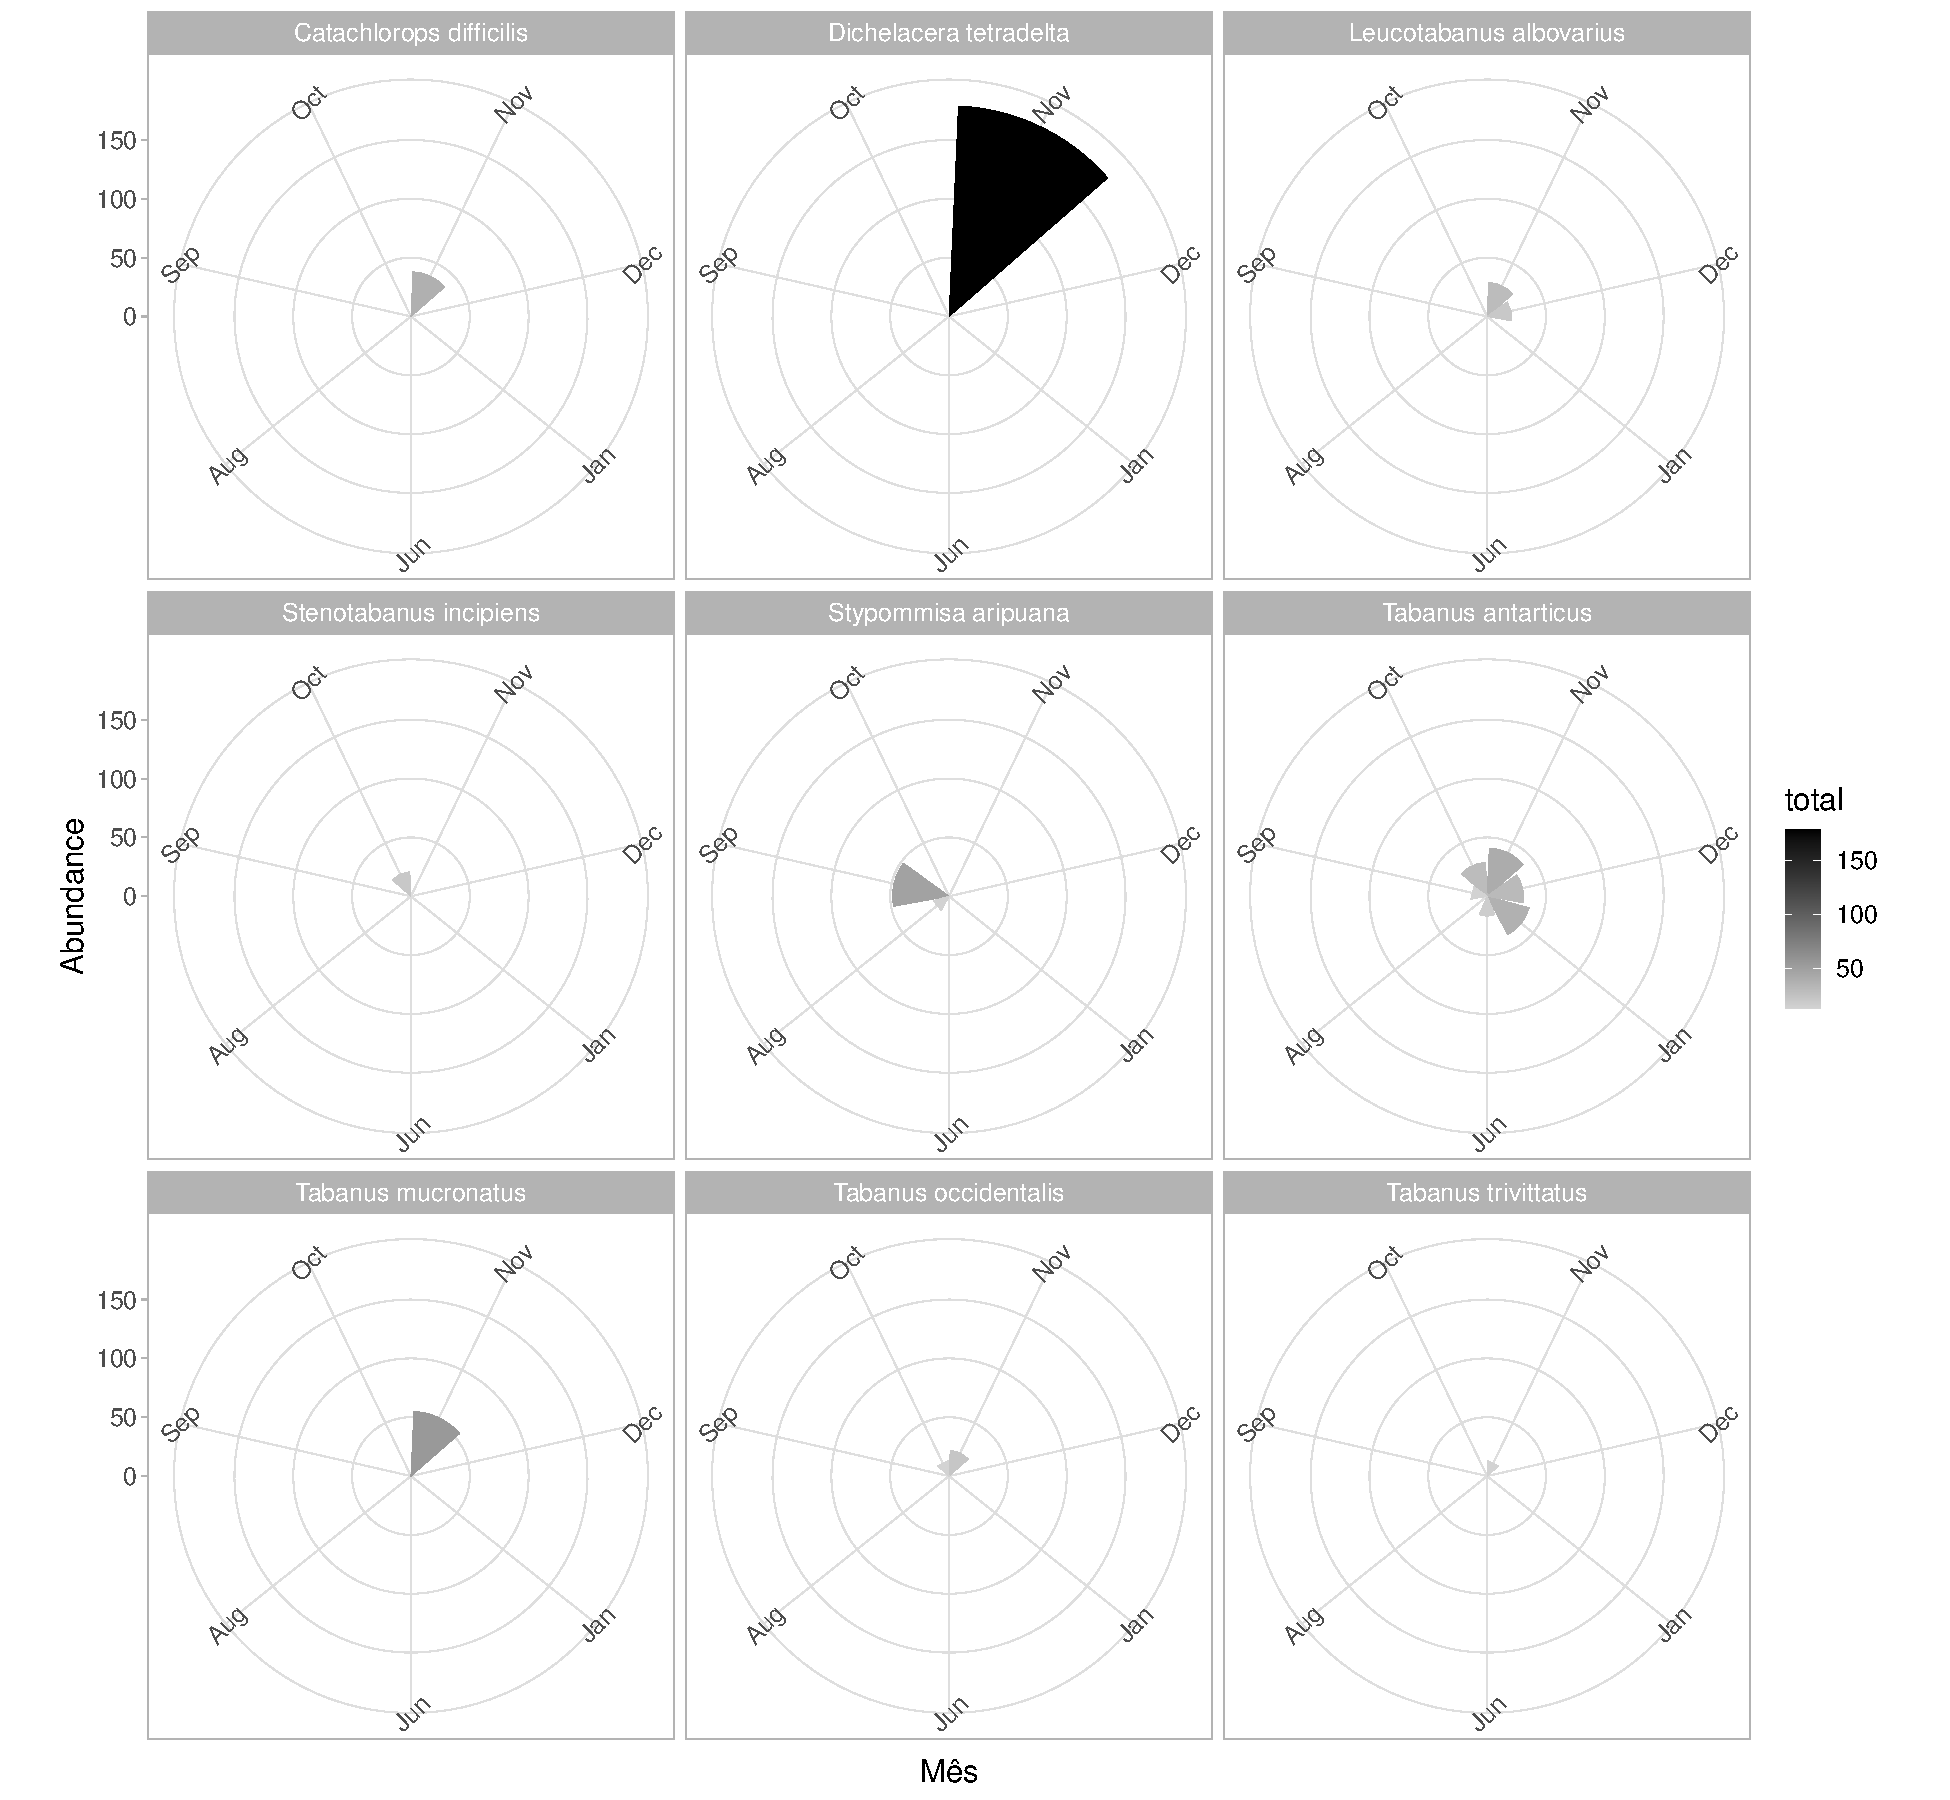
\includegraphics{report_nmds_files/figure-pdf/unnamed-chunk-3-1.pdf}

}

\end{figure}

\hypertarget{dataset-nmds}{%
\subsection{Dataset NMDS}\label{dataset-nmds}}

\begin{Shaded}
\begin{Highlighting}[]
\NormalTok{rich }\OtherTok{\textless{}{-}}
\NormalTok{  df  }\SpecialCharTok{\%\textgreater{}\%}
  \FunctionTok{group\_by}\NormalTok{(Localidade, Mês) }\SpecialCharTok{\%\textgreater{}\%}
  \FunctionTok{summarise}\NormalTok{(}\AttributeTok{rich =} \FunctionTok{n\_distinct}\NormalTok{(Espécie))}
\end{Highlighting}
\end{Shaded}

\begin{verbatim}
`summarise()` has grouped output by 'Localidade'. You can override using the
`.groups` argument.
\end{verbatim}

\begin{Shaded}
\begin{Highlighting}[]
\NormalTok{data\_nmds }\OtherTok{\textless{}{-}} 
\NormalTok{  df }\SpecialCharTok{\%\textgreater{}\%}
  \FunctionTok{group\_by}\NormalTok{(Espécie, Localidade, Mês) }\SpecialCharTok{\%\textgreater{}\%}
  \FunctionTok{summarise}\NormalTok{(}\AttributeTok{abund =} \FunctionTok{n}\NormalTok{()) }\SpecialCharTok{\%\textgreater{}\%}
  \FunctionTok{pivot\_wider}\NormalTok{(}\AttributeTok{names\_from =}\NormalTok{ Espécie, }\AttributeTok{values\_from =}\NormalTok{ abund) }\SpecialCharTok{\%\textgreater{}\%}
  \FunctionTok{replace}\NormalTok{(}\FunctionTok{is.na}\NormalTok{(.), }\DecValTok{0}\NormalTok{) }\SpecialCharTok{\%\textgreater{}\%}
  \FunctionTok{left\_join}\NormalTok{(rich, }\AttributeTok{by =} \FunctionTok{c}\NormalTok{(}\StringTok{"Localidade"}\NormalTok{, }\StringTok{"Mês"}\NormalTok{))}
\end{Highlighting}
\end{Shaded}

\begin{verbatim}
`summarise()` has grouped output by 'Espécie', 'Localidade'. You can override
using the `.groups` argument.
\end{verbatim}

\hypertarget{riqueza-e-abunduxe2ncia}{%
\subsection{RIQUEZA E ABUNDÂNCIA}\label{riqueza-e-abunduxe2ncia}}

\begin{Shaded}
\begin{Highlighting}[]
\NormalTok{rich\_abund }\OtherTok{\textless{}{-}} 
\NormalTok{  df }\SpecialCharTok{\%\textgreater{}\%}
  \FunctionTok{group\_by}\NormalTok{(Mês) }\SpecialCharTok{\%\textgreater{}\%}
  \FunctionTok{summarise}\NormalTok{(}\AttributeTok{rich =} \FunctionTok{n\_distinct}\NormalTok{(}\StringTok{\textasciigrave{}}\AttributeTok{Espécie}\StringTok{\textasciigrave{}}\NormalTok{),}
            \AttributeTok{abund =} \FunctionTok{n}\NormalTok{())}

\FunctionTok{ggplot}\NormalTok{(rich\_abund, }\FunctionTok{aes}\NormalTok{(}\AttributeTok{x =}\NormalTok{ abund, }\AttributeTok{y =}\NormalTok{ rich)) }\SpecialCharTok{+}
  \FunctionTok{geom\_point}\NormalTok{() }\SpecialCharTok{+}
  \FunctionTok{xlab}\NormalTok{(}\StringTok{\textquotesingle{}Abundance\textquotesingle{}}\NormalTok{) }\SpecialCharTok{+}
  \FunctionTok{ylab}\NormalTok{(}\StringTok{\textquotesingle{}Richness\textquotesingle{}}\NormalTok{) }\SpecialCharTok{+}
  \FunctionTok{geom\_smooth}\NormalTok{(}\AttributeTok{method =} \StringTok{"glm"}\NormalTok{, }\AttributeTok{alpha =}\NormalTok{ .}\DecValTok{15}\NormalTok{) }
\end{Highlighting}
\end{Shaded}

\begin{verbatim}
`geom_smooth()` using formula = 'y ~ x'
\end{verbatim}

\begin{figure}[H]

{\centering 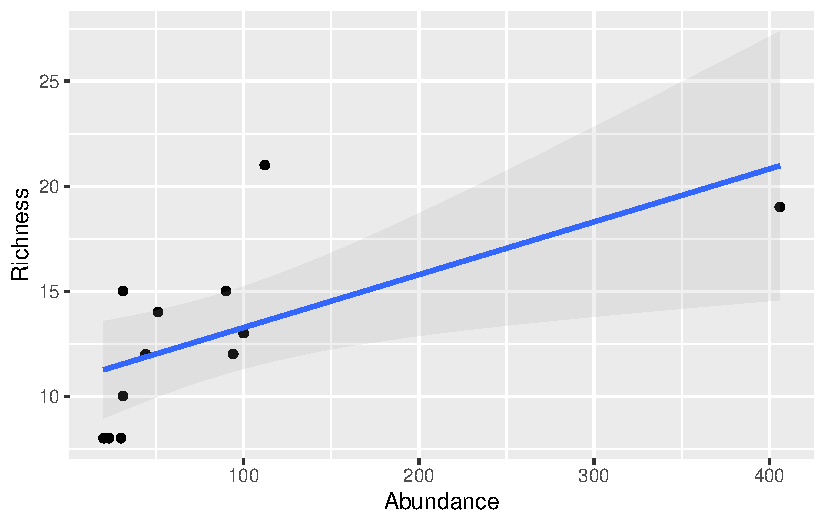
\includegraphics{report_nmds_files/figure-pdf/unnamed-chunk-5-1.pdf}

}

\end{figure}

\hypertarget{temperatura-umidade.-pressuxe3o-orvalho}{%
\subsection{TEMPERATURA, UMIDADE. PRESSÃO,
ORVALHO}\label{temperatura-umidade.-pressuxe3o-orvalho}}

\begin{Shaded}
\begin{Highlighting}[]
\NormalTok{df\_climatics }\OtherTok{\textless{}{-}} 
\NormalTok{  df }\SpecialCharTok{\%\textgreater{}\%} 
  \FunctionTok{group\_by}\NormalTok{(Mês) }\SpecialCharTok{\%\textgreater{}\%}
  \FunctionTok{summarise}\NormalTok{(}
    \AttributeTok{abund =} \FunctionTok{n}\NormalTok{(),}
    \AttributeTok{temp =} \FunctionTok{mean}\NormalTok{(}\FunctionTok{as.numeric}\NormalTok{(}\StringTok{\textasciigrave{}}\AttributeTok{Temperatura média (°C)}\StringTok{\textasciigrave{}}\NormalTok{)),}
    \AttributeTok{um =} \FunctionTok{mean}\NormalTok{(}\FunctionTok{as.numeric}\NormalTok{(}\StringTok{\textasciigrave{}}\AttributeTok{Umidade média (\%)}\StringTok{\textasciigrave{}}\NormalTok{)),}
    \AttributeTok{or =} \FunctionTok{mean}\NormalTok{(}\FunctionTok{as.numeric}\NormalTok{(}\StringTok{\textasciigrave{}}\AttributeTok{Pto. Orvalho média (°C)}\StringTok{\textasciigrave{}}\NormalTok{)),}
    \AttributeTok{pre =} \FunctionTok{mean}\NormalTok{(}\FunctionTok{as.numeric}\NormalTok{(}\StringTok{\textasciigrave{}}\AttributeTok{Pressão média (hPa)}\StringTok{\textasciigrave{}}\NormalTok{)),}
    \AttributeTok{rich =} \FunctionTok{n\_distinct}\NormalTok{(}\StringTok{\textasciigrave{}}\AttributeTok{Espécie}\StringTok{\textasciigrave{}}\NormalTok{)}
\NormalTok{  )}

\NormalTok{df\_climatics[}\DecValTok{4}\NormalTok{,}\DecValTok{3}\NormalTok{] }\OtherTok{\textless{}{-}} \FloatTok{25.36}
\end{Highlighting}
\end{Shaded}

\begin{Shaded}
\begin{Highlighting}[]
\FunctionTok{ggplot}\NormalTok{(df\_climatics, }\FunctionTok{aes}\NormalTok{(}\AttributeTok{x =}\NormalTok{ temp, }\AttributeTok{y =}\NormalTok{ abund)) }\SpecialCharTok{+}
  \FunctionTok{geom\_point}\NormalTok{() }\SpecialCharTok{+}
  \FunctionTok{geom\_smooth}\NormalTok{(}\AttributeTok{method =} \StringTok{"lm"}\NormalTok{, }\AttributeTok{alpha =}\NormalTok{ .}\DecValTok{15}\NormalTok{)}
\end{Highlighting}
\end{Shaded}

\begin{verbatim}
`geom_smooth()` using formula = 'y ~ x'
\end{verbatim}

\begin{figure}[H]

{\centering 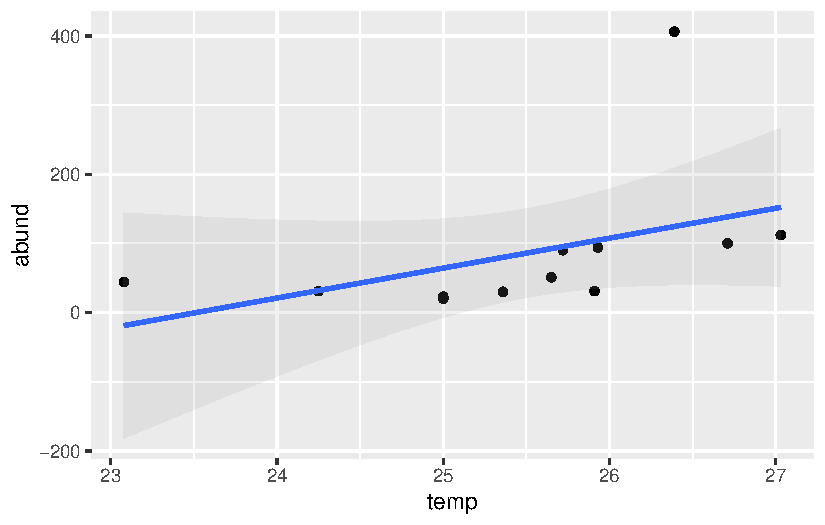
\includegraphics{report_nmds_files/figure-pdf/unnamed-chunk-7-1.pdf}

}

\end{figure}

\begin{Shaded}
\begin{Highlighting}[]
\FunctionTok{ggplot}\NormalTok{(df\_climatics, }\FunctionTok{aes}\NormalTok{(}\AttributeTok{x =}\NormalTok{ um, }\AttributeTok{y =}\NormalTok{ abund)) }\SpecialCharTok{+}
  \FunctionTok{geom\_point}\NormalTok{() }\SpecialCharTok{+}
  \FunctionTok{geom\_smooth}\NormalTok{(}\AttributeTok{method =} \StringTok{"lm"}\NormalTok{, }\AttributeTok{alpha =}\NormalTok{ .}\DecValTok{15}\NormalTok{)}
\end{Highlighting}
\end{Shaded}

\begin{verbatim}
`geom_smooth()` using formula = 'y ~ x'
\end{verbatim}

\begin{figure}[H]

{\centering 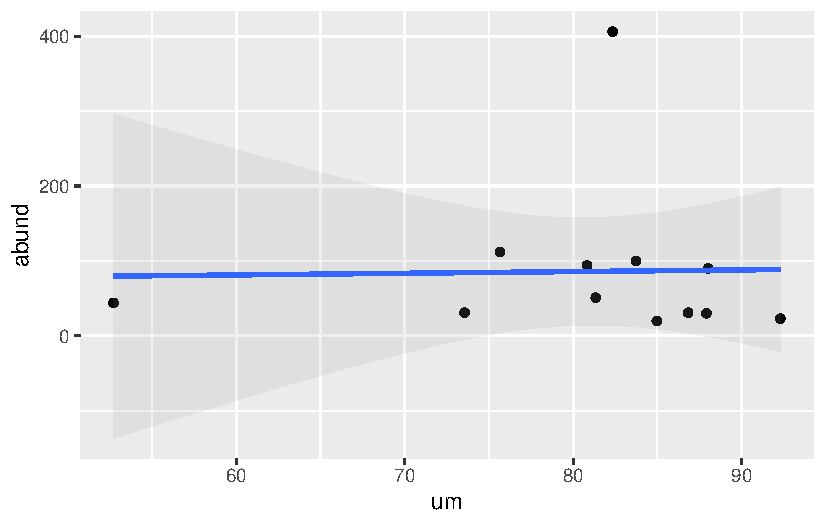
\includegraphics{report_nmds_files/figure-pdf/unnamed-chunk-8-1.pdf}

}

\end{figure}

\begin{Shaded}
\begin{Highlighting}[]
\FunctionTok{ggplot}\NormalTok{(df\_climatics, }\FunctionTok{aes}\NormalTok{(}\AttributeTok{x =}\NormalTok{ or, }\AttributeTok{y =}\NormalTok{ abund)) }\SpecialCharTok{+}
  \FunctionTok{geom\_point}\NormalTok{() }\SpecialCharTok{+}
  \FunctionTok{geom\_smooth}\NormalTok{(}\AttributeTok{method =} \StringTok{"lm"}\NormalTok{, }\AttributeTok{alpha =}\NormalTok{ .}\DecValTok{15}\NormalTok{)}
\end{Highlighting}
\end{Shaded}

\begin{verbatim}
`geom_smooth()` using formula = 'y ~ x'
\end{verbatim}

\begin{figure}[H]

{\centering 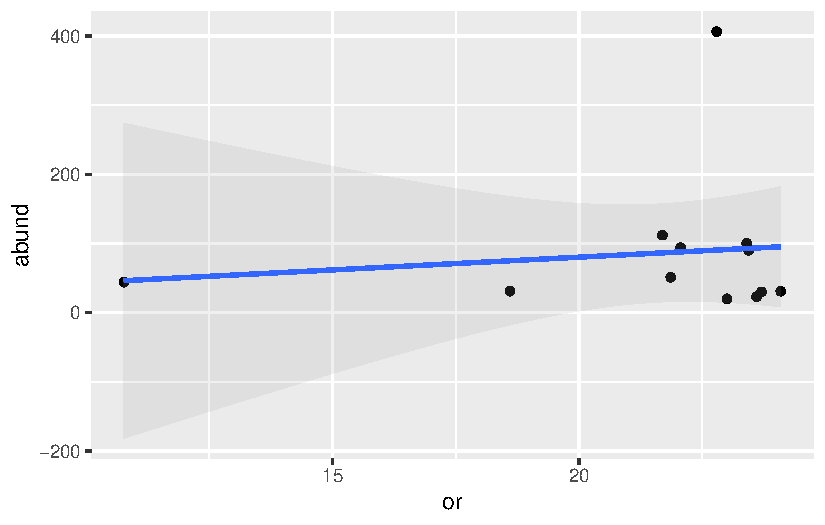
\includegraphics{report_nmds_files/figure-pdf/unnamed-chunk-9-1.pdf}

}

\end{figure}

\begin{Shaded}
\begin{Highlighting}[]
\FunctionTok{ggplot}\NormalTok{(df\_climatics, }\FunctionTok{aes}\NormalTok{(}\AttributeTok{x =}\NormalTok{ pre, }\AttributeTok{y =}\NormalTok{ abund)) }\SpecialCharTok{+}
  \FunctionTok{geom\_point}\NormalTok{() }\SpecialCharTok{+}
  \FunctionTok{geom\_smooth}\NormalTok{(}\AttributeTok{method =} \StringTok{"lm"}\NormalTok{, }\AttributeTok{alpha =}\NormalTok{ .}\DecValTok{15}\NormalTok{)}
\end{Highlighting}
\end{Shaded}

\begin{verbatim}
`geom_smooth()` using formula = 'y ~ x'
\end{verbatim}

\begin{figure}[H]

{\centering 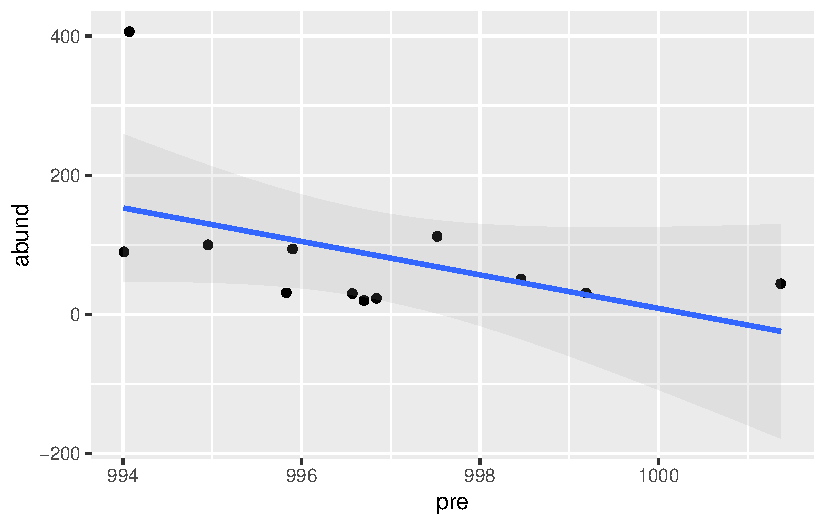
\includegraphics{report_nmds_files/figure-pdf/unnamed-chunk-10-1.pdf}

}

\end{figure}

\hypertarget{riqueza-e-abunduxe2ncia-por-muxeas}{%
\subsection{RIQUEZA e ABUNDÂNCIA POR
MÊS}\label{riqueza-e-abunduxe2ncia-por-muxeas}}

\begin{Shaded}
\begin{Highlighting}[]
\FunctionTok{ggplot}\NormalTok{(df\_climatics, }\FunctionTok{aes}\NormalTok{(}\AttributeTok{x =}\NormalTok{ temp , }\AttributeTok{y =}\NormalTok{ rich)) }\SpecialCharTok{+}
  \FunctionTok{geom\_point}\NormalTok{() }\SpecialCharTok{+}
  \FunctionTok{geom\_smooth}\NormalTok{(}\AttributeTok{method=}\StringTok{"glm"}\NormalTok{, }\AttributeTok{family=}\StringTok{"poisson"}\NormalTok{, }\AttributeTok{se=}\ConstantTok{TRUE}\NormalTok{)}
\end{Highlighting}
\end{Shaded}

\begin{verbatim}
Warning in geom_smooth(method = "glm", family = "poisson", se = TRUE): Ignoring
unknown parameters: `family`
\end{verbatim}

\begin{verbatim}
`geom_smooth()` using formula = 'y ~ x'
\end{verbatim}

\begin{figure}[H]

{\centering 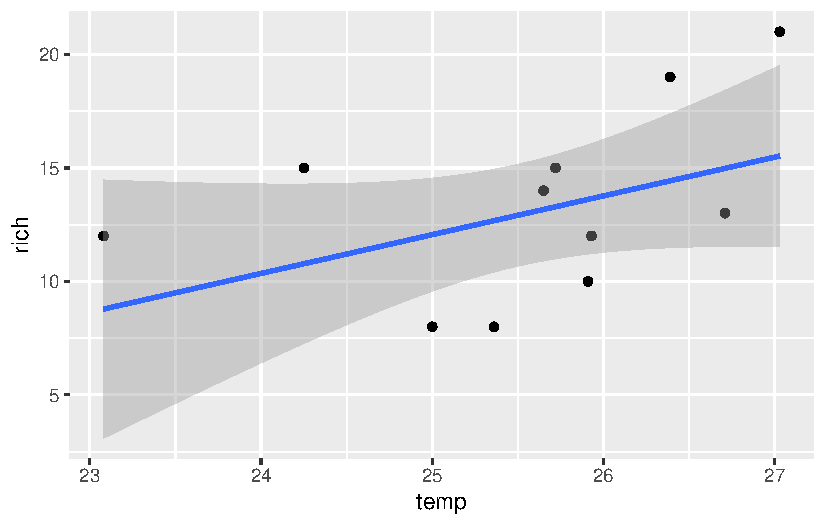
\includegraphics{report_nmds_files/figure-pdf/unnamed-chunk-11-1.pdf}

}

\end{figure}

\begin{Shaded}
\begin{Highlighting}[]
\NormalTok{model1 }\OtherTok{\textless{}{-}} \FunctionTok{glm}\NormalTok{(}\AttributeTok{data =}\NormalTok{ df\_climatics, }
\NormalTok{              rich }\SpecialCharTok{\textasciitilde{}}\NormalTok{ temp}\SpecialCharTok{*}\NormalTok{um}\SpecialCharTok{*}\NormalTok{or}\SpecialCharTok{*}\NormalTok{pre, }\AttributeTok{family =} \StringTok{\textquotesingle{}poisson\textquotesingle{}}\NormalTok{)}

\FunctionTok{summary}\NormalTok{(model1)}
\end{Highlighting}
\end{Shaded}

\begin{verbatim}

Call:
glm(formula = rich ~ temp * um * or * pre, family = "poisson", 
    data = df_climatics)

Deviance Residuals: 
 [1]  0  0  0  0  0  0  0  0  0  0  0  0

Coefficients: (4 not defined because of singularities)
                 Estimate Std. Error z value Pr(>|z|)
(Intercept)    -3.533e+03  2.590e+04  -0.136    0.891
temp           -1.251e+02  1.161e+03  -0.108    0.914
um             -9.832e+01  2.523e+02  -0.390    0.697
or              7.009e+02  1.170e+03   0.599    0.549
pre             3.018e+00  2.562e+01   0.118    0.906
temp:um        -6.071e-02  2.961e-01  -0.205    0.838
temp:or        -1.034e+00  2.257e+00  -0.458    0.647
um:or          -1.150e-01  3.950e-01  -0.291    0.771
temp:pre        1.461e-01  1.146e+00   0.128    0.899
um:pre          1.003e-01  2.536e-01   0.395    0.692
or:pre         -6.767e-01  1.189e+00  -0.569    0.569
temp:um:or      4.343e-03  1.869e-02   0.232    0.816
temp:um:pre            NA         NA      NA       NA
temp:or:pre            NA         NA      NA       NA
um:or:pre              NA         NA      NA       NA
temp:um:or:pre         NA         NA      NA       NA

(Dispersion parameter for poisson family taken to be 1)

    Null deviance: 1.4824e+01  on 11  degrees of freedom
Residual deviance: 6.6613e-15  on  0  degrees of freedom
AIC: 76.345

Number of Fisher Scoring iterations: 3
\end{verbatim}

\begin{Shaded}
\begin{Highlighting}[]
\FunctionTok{anova}\NormalTok{(model1, }\AttributeTok{test =} \StringTok{\textquotesingle{}Chisq\textquotesingle{}}\NormalTok{)}
\end{Highlighting}
\end{Shaded}

\begin{verbatim}
Analysis of Deviance Table

Model: poisson, link: log

Response: rich

Terms added sequentially (first to last)

               Df Deviance Resid. Df Resid. Dev Pr(>Chi)  
NULL                              11    14.8236           
temp            1   3.0356        10    11.7880  0.08145 .
um              1   5.8717         9     5.9162  0.01539 *
or              1   0.2309         8     5.6853  0.63085  
pre             1   0.1827         7     5.5027  0.66910  
temp:um         1   2.6998         6     2.8029  0.10036  
temp:or         1   0.3990         5     2.4039  0.52762  
um:or           1   0.2062         4     2.1977  0.64972  
temp:pre        1   0.0503         3     2.1474  0.82254  
um:pre          1   1.6047         2     0.5427  0.20524  
or:pre          1   0.4886         1     0.0541  0.48456  
temp:um:or      1   0.0541         0     0.0000  0.81612  
temp:um:pre     0   0.0000         0     0.0000           
temp:or:pre     0   0.0000         0     0.0000           
um:or:pre       0   0.0000         0     0.0000           
temp:um:or:pre  0   0.0000         0     0.0000           
---
Signif. codes:  0 '***' 0.001 '**' 0.01 '*' 0.05 '.' 0.1 ' ' 1
\end{verbatim}

\hypertarget{diversidade}{%
\subsection{DIVERSIDADE}\label{diversidade}}

\begin{Shaded}
\begin{Highlighting}[]
\NormalTok{abund }\OtherTok{\textless{}{-}}\NormalTok{ df }\SpecialCharTok{\%\textgreater{}\%}
  \FunctionTok{group\_by}\NormalTok{(Espécie, Localidade) }\SpecialCharTok{\%\textgreater{}\%}
  \FunctionTok{summarise}\NormalTok{(}\AttributeTok{total =} \FunctionTok{n}\NormalTok{()) }\SpecialCharTok{\%\textgreater{}\%}
  \FunctionTok{pivot\_wider}\NormalTok{(}\AttributeTok{names\_from =}\NormalTok{ Localidade, }\AttributeTok{values\_from =}\NormalTok{ total)  }\SpecialCharTok{\%\textgreater{}\%}
  \FunctionTok{replace\_na}\NormalTok{(}\FunctionTok{list}\NormalTok{(}\StringTok{\textasciigrave{}}\AttributeTok{P1 {-} Argeu}\StringTok{\textasciigrave{}} \OtherTok{=} \DecValTok{0}\NormalTok{, }\StringTok{\textasciigrave{}}\AttributeTok{P2 {-} Hélio}\StringTok{\textasciigrave{}} \OtherTok{=} \DecValTok{0}\NormalTok{, }\StringTok{\textasciigrave{}}\AttributeTok{P3 {-} Paulo Cabeça}\StringTok{\textasciigrave{}} \OtherTok{=} \DecValTok{0}\NormalTok{,}
                  \StringTok{\textasciigrave{}}\AttributeTok{P4 {-} Paulo Vicentino}\StringTok{\textasciigrave{}} \OtherTok{=} \DecValTok{0}\NormalTok{, }\StringTok{\textasciigrave{}}\AttributeTok{P5 {-} Nelcivaldo}\StringTok{\textasciigrave{}} \OtherTok{=} \DecValTok{0}\NormalTok{)) }\SpecialCharTok{\%\textgreater{}\%}
  \FunctionTok{column\_to\_rownames}\NormalTok{(}\AttributeTok{var =} \StringTok{"Espécie"}\NormalTok{)}
\end{Highlighting}
\end{Shaded}

\begin{verbatim}
`summarise()` has grouped output by 'Espécie'. You can override using the
`.groups` argument.
\end{verbatim}

\begin{Shaded}
\begin{Highlighting}[]
\NormalTok{resultados\_tabanidae }\OtherTok{\textless{}{-}} \FunctionTok{iNEXT}\NormalTok{(abund,}
                              \AttributeTok{q =} \DecValTok{0}\NormalTok{,}
                              \AttributeTok{datatype =} \StringTok{"abundance"}\NormalTok{,}
                              \AttributeTok{endpoint =} \DecValTok{400}
\NormalTok{)}
\end{Highlighting}
\end{Shaded}

\begin{Shaded}
\begin{Highlighting}[]
\NormalTok{resultados\_tabanidae}\SpecialCharTok{$}\NormalTok{AsyEst}
\end{Highlighting}
\end{Shaded}

\begin{verbatim}
             Assemblage         Diversity  Observed Estimator       s.e.
1            P1 - Argeu  Species richness 29.000000 31.563843  8.6250670
2            P1 - Argeu Shannon diversity 12.801577 13.453947  0.8035587
3            P1 - Argeu Simpson diversity  9.000000  9.218182  0.5830456
4            P2 - Hélio  Species richness 16.000000 33.842105 11.6128384
5            P2 - Hélio Shannon diversity  7.855252  8.963119  1.1236311
6            P2 - Hélio Simpson diversity  4.871064  5.043853  0.7723770
7     P3 - Paulo Cabeça  Species richness 12.000000 13.967742  5.0082908
8     P3 - Paulo Cabeça Shannon diversity  6.248792  7.045848  1.0106187
9     P3 - Paulo Cabeça Simpson diversity  4.261641  4.502381  0.7957198
10 P4 - Paulo Vicentino  Species richness 19.000000 25.080935 12.4875083
11 P4 - Paulo Vicentino Shannon diversity  6.035785  6.657075  0.9459506
12 P4 - Paulo Vicentino Simpson diversity  3.123848  3.172676  0.4184061
13      P5 - Nelcivaldo  Species richness 31.000000 40.973545 11.7648417
14      P5 - Nelcivaldo Shannon diversity  8.493632  9.006481  0.6568116
15      P5 - Nelcivaldo Simpson diversity  4.931456  4.983424  0.3265694
         LCL       UCL
1  29.000000 48.468664
2  11.879000 15.028893
3   8.075433 10.360930
4  16.000000 56.602850
5   6.760843 11.165396
6   3.530022  6.557684
7  12.000000 23.783812
8   5.065072  9.026625
9   2.942799  6.061963
10 19.000000 49.556002
11  4.803046  8.511104
12  2.352615  3.992737
13 31.000000 64.032211
14  7.719154 10.293808
15  4.343360  5.623488
\end{verbatim}

\begin{Shaded}
\begin{Highlighting}[]
\FunctionTok{ggiNEXT}\NormalTok{(resultados\_tabanidae, }\AttributeTok{type =} \DecValTok{1}\NormalTok{, }\AttributeTok{facet.var =} \StringTok{\textquotesingle{}Order\textquotesingle{}}\NormalTok{) }\SpecialCharTok{+} 
  \FunctionTok{theme\_light}\NormalTok{() }
\end{Highlighting}
\end{Shaded}

\begin{verbatim}
Warning in ggiNEXT.iNEXT(resultados_tabanidae, type = 1, facet.var = "Order"):
invalid facet.var setting, the iNEXT object do not consist multiple orders.
\end{verbatim}

\begin{figure}[H]

{\centering 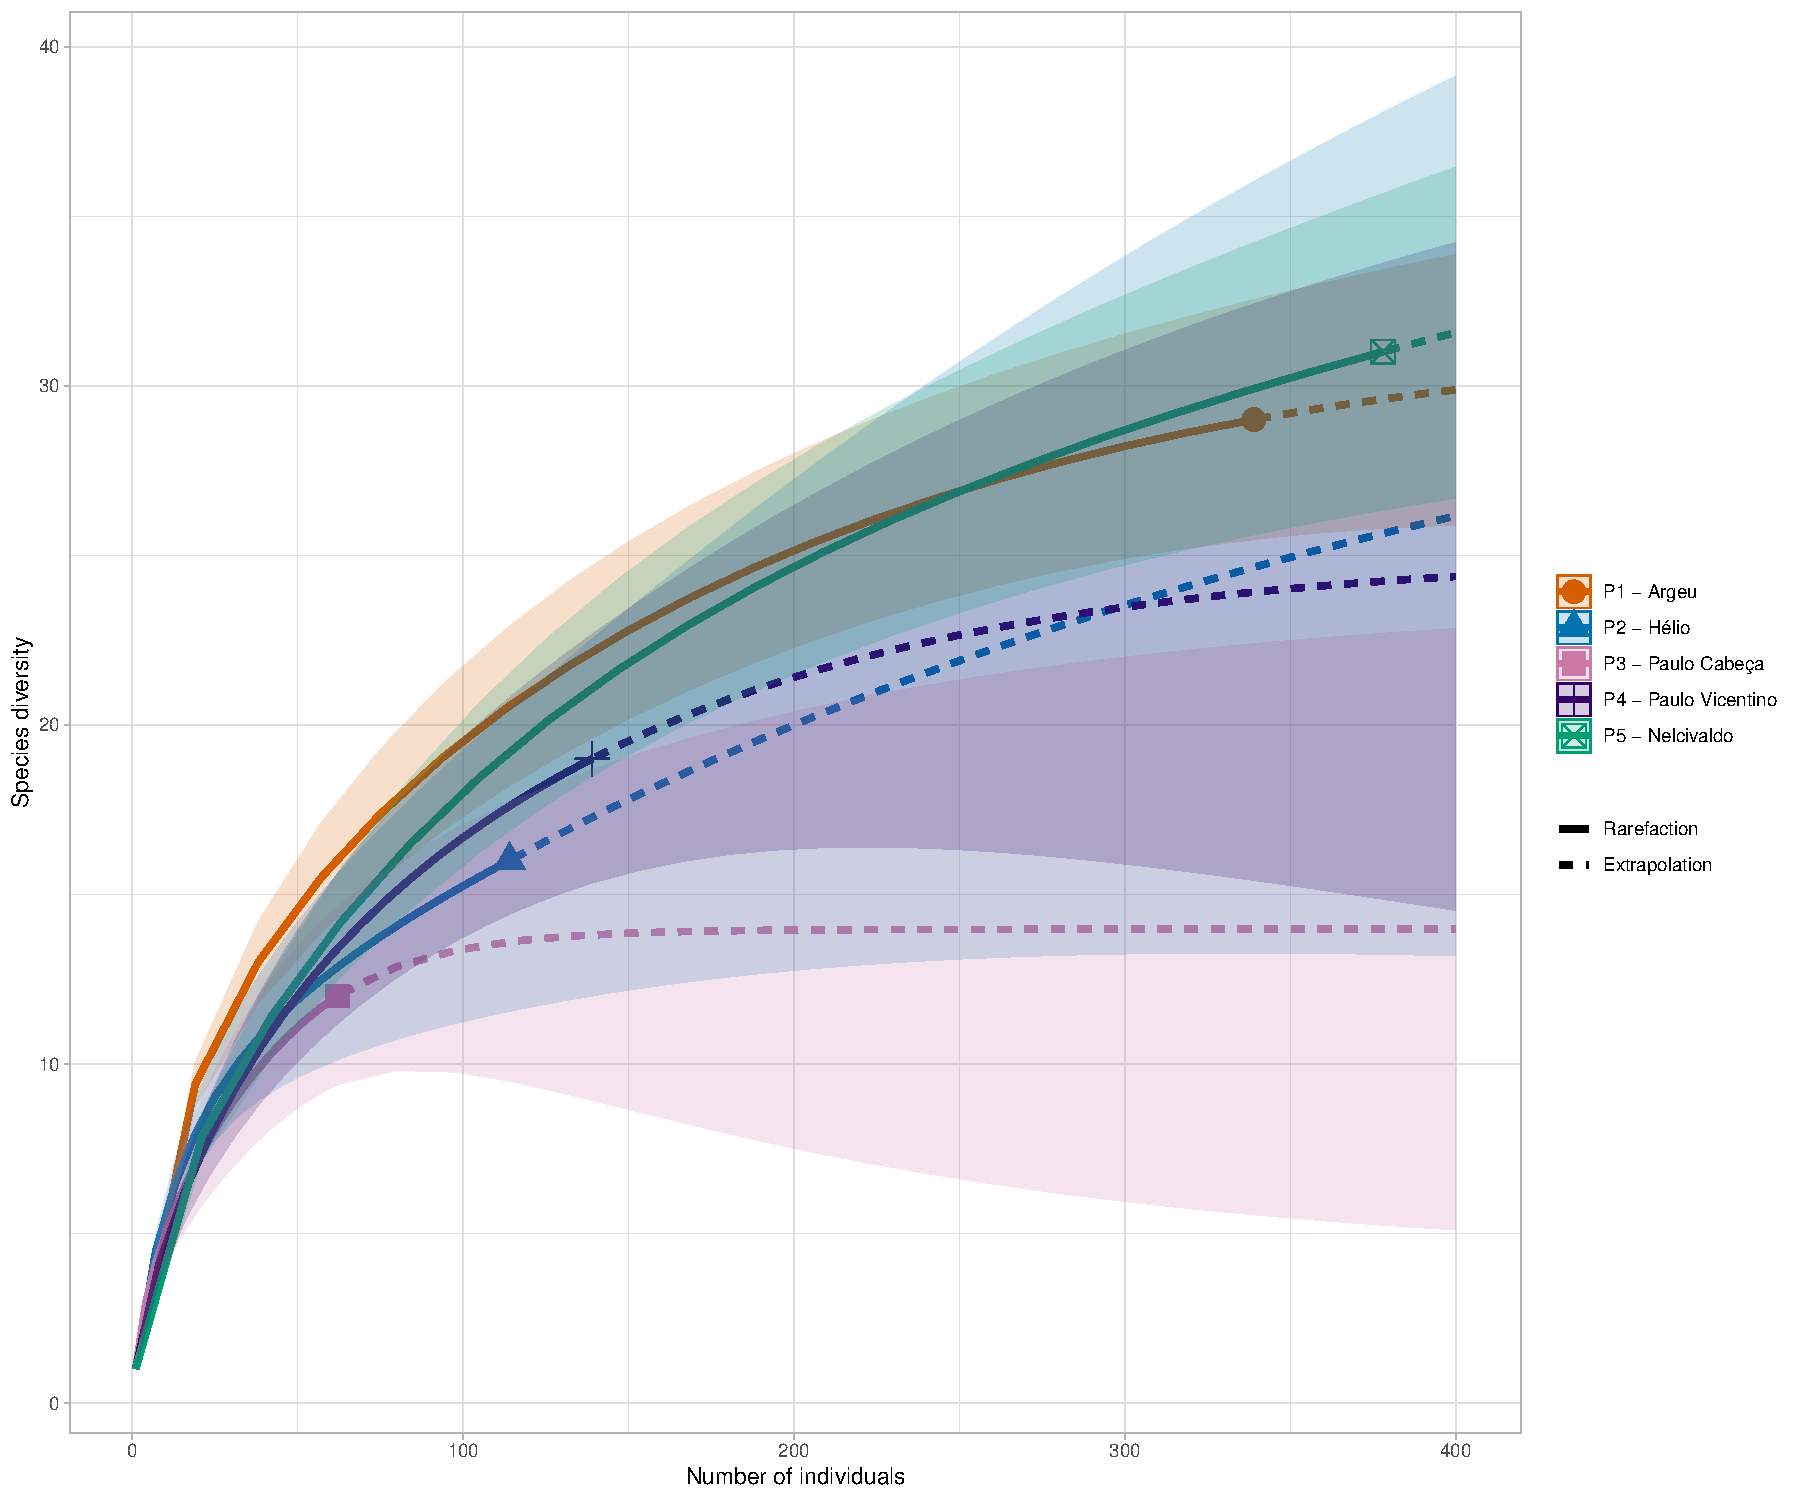
\includegraphics{report_nmds_files/figure-pdf/unnamed-chunk-15-1.pdf}

}

\end{figure}

\hypertarget{upgma}{%
\subsection{UPGMA}\label{upgma}}

\hypertarget{localidade}{%
\subsubsection{Localidade}\label{localidade}}

\begin{Shaded}
\begin{Highlighting}[]
\NormalTok{env\_df }\OtherTok{\textless{}{-}}\NormalTok{ df }\SpecialCharTok{\%\textgreater{}\%} 
  \FunctionTok{group\_by}\NormalTok{(Localidade, Espécie) }\SpecialCharTok{\%\textgreater{}\%}
  \FunctionTok{summarise}\NormalTok{(}\AttributeTok{abund =} \FunctionTok{n}\NormalTok{()) }\SpecialCharTok{\%\textgreater{}\%}
  \FunctionTok{pivot\_wider}\NormalTok{(}\AttributeTok{names\_from =}\NormalTok{ Espécie, }
              \AttributeTok{values\_from =}\NormalTok{ abund) }\SpecialCharTok{\%\textgreater{}\%}\FunctionTok{replace}\NormalTok{(}\FunctionTok{is.na}\NormalTok{(.), }\DecValTok{0}\NormalTok{)}
\end{Highlighting}
\end{Shaded}

\begin{verbatim}
`summarise()` has grouped output by 'Localidade'. You can override using the
`.groups` argument.
\end{verbatim}

\begin{Shaded}
\begin{Highlighting}[]
\NormalTok{especies }\OtherTok{\textless{}{-}}\NormalTok{ env\_df[ ,}\DecValTok{3}\SpecialCharTok{:}\DecValTok{47}\NormalTok{]}
\NormalTok{dist.bray }\OtherTok{\textless{}{-}} \FunctionTok{vegdist}\NormalTok{(especies, }\AttributeTok{method =} \StringTok{"bray"}\NormalTok{)}
\NormalTok{cluster.bray }\OtherTok{\textless{}{-}} \FunctionTok{hclust}\NormalTok{(dist.bray, }\AttributeTok{method =} \StringTok{"average"}\NormalTok{)}

\NormalTok{cluster.bray}\SpecialCharTok{$}\NormalTok{labels }\OtherTok{\textless{}{-}}\NormalTok{env\_df}\SpecialCharTok{$}\NormalTok{Localidade}

\NormalTok{cluster2.bray }\OtherTok{\textless{}{-}} \FunctionTok{as.dendrogram}\NormalTok{(cluster.bray)}
\FunctionTok{par}\NormalTok{(}\AttributeTok{mar=}\FunctionTok{c}\NormalTok{(}\DecValTok{2}\NormalTok{,}\DecValTok{2}\NormalTok{,}\DecValTok{2}\NormalTok{,}\DecValTok{15}\NormalTok{))}
\FunctionTok{plot}\NormalTok{(cluster2.bray, }\AttributeTok{horiz =} \ConstantTok{TRUE}\NormalTok{, }\AttributeTok{xlab =} \StringTok{"Dissimilarity Indices"}\NormalTok{)}
\end{Highlighting}
\end{Shaded}

\begin{figure}[H]

{\centering 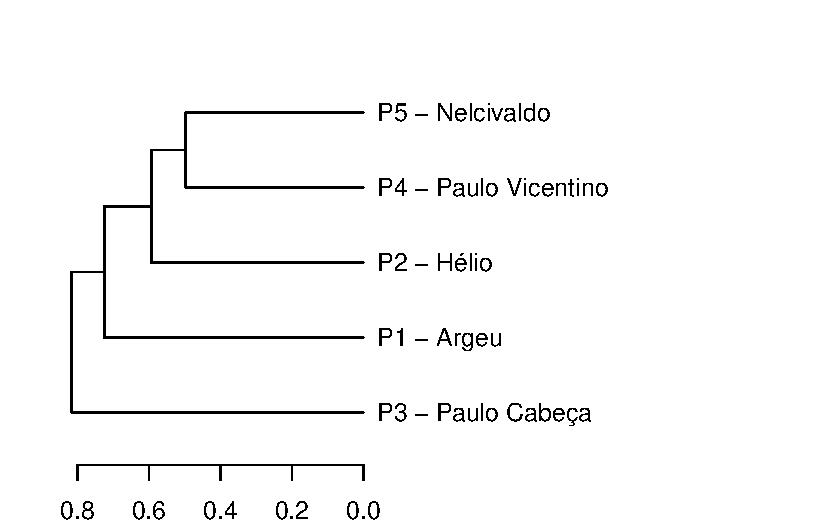
\includegraphics{report_nmds_files/figure-pdf/unnamed-chunk-17-1.pdf}

}

\end{figure}

\hypertarget{armadilha}{%
\subsubsection{Armadilha}\label{armadilha}}

\begin{Shaded}
\begin{Highlighting}[]
\NormalTok{env\_df }\OtherTok{\textless{}{-}}\NormalTok{ df }\SpecialCharTok{\%\textgreater{}\%} 
  \FunctionTok{group\_by}\NormalTok{(Armadilha, Espécie) }\SpecialCharTok{\%\textgreater{}\%}
  \FunctionTok{summarise}\NormalTok{(}\AttributeTok{abund =} \FunctionTok{n}\NormalTok{()) }\SpecialCharTok{\%\textgreater{}\%}
  \FunctionTok{pivot\_wider}\NormalTok{(}\AttributeTok{names\_from =}\NormalTok{ Espécie, }
              \AttributeTok{values\_from =}\NormalTok{ abund) }\SpecialCharTok{\%\textgreater{}\%}\FunctionTok{replace}\NormalTok{(}\FunctionTok{is.na}\NormalTok{(.), }\DecValTok{0}\NormalTok{)}
\end{Highlighting}
\end{Shaded}

\begin{verbatim}
`summarise()` has grouped output by 'Armadilha'. You can override using the
`.groups` argument.
\end{verbatim}

\begin{Shaded}
\begin{Highlighting}[]
\NormalTok{especies }\OtherTok{\textless{}{-}}\NormalTok{ env\_df[ ,}\DecValTok{3}\SpecialCharTok{:}\DecValTok{47}\NormalTok{]}
\CommentTok{\#não é necessário padronização, pois a abundância de espécies esta em mesma escala}
\NormalTok{dist.bray }\OtherTok{\textless{}{-}} \FunctionTok{vegdist}\NormalTok{(especies, }\AttributeTok{method =} \StringTok{"bray"}\NormalTok{)}
\NormalTok{cluster.bray }\OtherTok{\textless{}{-}} \FunctionTok{hclust}\NormalTok{(dist.bray, }\AttributeTok{method =} \StringTok{"average"}\NormalTok{)}

\NormalTok{cluster.bray}\SpecialCharTok{$}\NormalTok{labels }\OtherTok{\textless{}{-}}\NormalTok{ env\_df}\SpecialCharTok{$}\NormalTok{Armadilha}

\NormalTok{cluster2.bray }\OtherTok{\textless{}{-}} \FunctionTok{as.dendrogram}\NormalTok{(cluster.bray)}
\FunctionTok{par}\NormalTok{(}\AttributeTok{mar=}\FunctionTok{c}\NormalTok{(}\DecValTok{2}\NormalTok{,}\DecValTok{2}\NormalTok{,}\DecValTok{2}\NormalTok{,}\DecValTok{10}\NormalTok{))}
\FunctionTok{plot}\NormalTok{(cluster2.bray, }\AttributeTok{horiz =} \ConstantTok{TRUE}\NormalTok{, }\AttributeTok{xlab =} \StringTok{"Dissimilarity Indices"}\NormalTok{)}
\end{Highlighting}
\end{Shaded}

\begin{figure}[H]

{\centering 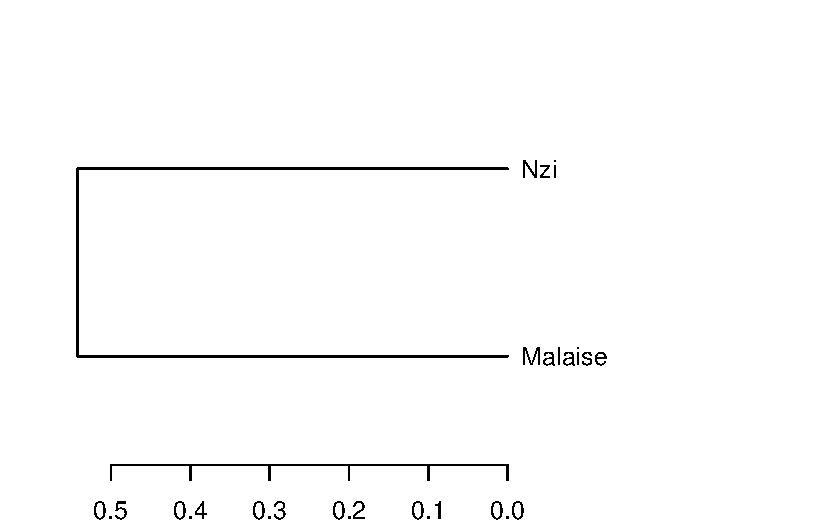
\includegraphics{report_nmds_files/figure-pdf/unnamed-chunk-19-1.pdf}

}

\end{figure}

\hypertarget{ambiente}{%
\subsubsection{Ambiente}\label{ambiente}}

\begin{Shaded}
\begin{Highlighting}[]
\NormalTok{env\_df }\OtherTok{\textless{}{-}}\NormalTok{ df }\SpecialCharTok{\%\textgreater{}\%} 
  \FunctionTok{group\_by}\NormalTok{(Ambiente, Espécie) }\SpecialCharTok{\%\textgreater{}\%}
  \FunctionTok{summarise}\NormalTok{(}\AttributeTok{abund =} \FunctionTok{n}\NormalTok{()) }\SpecialCharTok{\%\textgreater{}\%}
  \FunctionTok{pivot\_wider}\NormalTok{(}\AttributeTok{names\_from =}\NormalTok{ Espécie, }
              \AttributeTok{values\_from =}\NormalTok{ abund) }\SpecialCharTok{\%\textgreater{}\%}\FunctionTok{replace}\NormalTok{(}\FunctionTok{is.na}\NormalTok{(.), }\DecValTok{0}\NormalTok{)}
\end{Highlighting}
\end{Shaded}

\begin{verbatim}
`summarise()` has grouped output by 'Ambiente'. You can override using the
`.groups` argument.
\end{verbatim}

\begin{Shaded}
\begin{Highlighting}[]
\NormalTok{especies }\OtherTok{\textless{}{-}}\NormalTok{ env\_df[ ,}\DecValTok{3}\SpecialCharTok{:}\DecValTok{47}\NormalTok{]}
\CommentTok{\# não é necessário padronização, pois a abundância de espécies esta em mesma escala}
\NormalTok{dist.bray }\OtherTok{\textless{}{-}} \FunctionTok{vegdist}\NormalTok{(especies, }\AttributeTok{method =} \StringTok{"bray"}\NormalTok{)}
\NormalTok{cluster.bray }\OtherTok{\textless{}{-}} \FunctionTok{hclust}\NormalTok{(dist.bray, }\AttributeTok{method =} \StringTok{"average"}\NormalTok{)}

\NormalTok{cluster.bray}\SpecialCharTok{$}\NormalTok{labels }\OtherTok{\textless{}{-}}\NormalTok{ env\_df}\SpecialCharTok{$}\NormalTok{Ambiente}

\NormalTok{cluster2.bray }\OtherTok{\textless{}{-}} \FunctionTok{as.dendrogram}\NormalTok{(cluster.bray)}
\FunctionTok{par}\NormalTok{(}\AttributeTok{mar=}\FunctionTok{c}\NormalTok{(}\DecValTok{2}\NormalTok{,}\DecValTok{2}\NormalTok{,}\DecValTok{2}\NormalTok{,}\DecValTok{15}\NormalTok{))}
\FunctionTok{plot}\NormalTok{(cluster2.bray, }\AttributeTok{horiz =} \ConstantTok{TRUE}\NormalTok{, }\AttributeTok{xlab =} \StringTok{"Dissimilarity Indices"}\NormalTok{)}
\end{Highlighting}
\end{Shaded}

\begin{figure}[H]

{\centering 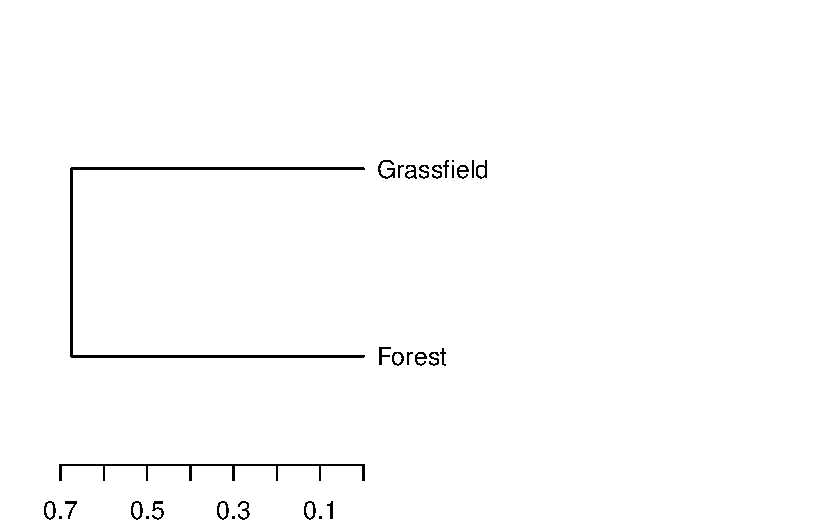
\includegraphics{report_nmds_files/figure-pdf/unnamed-chunk-21-1.pdf}

}

\end{figure}

\hypertarget{muxeas}{%
\subsubsection{Mês}\label{muxeas}}

\begin{Shaded}
\begin{Highlighting}[]
\NormalTok{env\_df }\OtherTok{\textless{}{-}}\NormalTok{ df }\SpecialCharTok{\%\textgreater{}\%} 
  \FunctionTok{group\_by}\NormalTok{(Mês, Espécie) }\SpecialCharTok{\%\textgreater{}\%}
  \FunctionTok{summarise}\NormalTok{(}\AttributeTok{abund =} \FunctionTok{n}\NormalTok{()) }\SpecialCharTok{\%\textgreater{}\%}
  \FunctionTok{pivot\_wider}\NormalTok{(}\AttributeTok{names\_from =}\NormalTok{ Espécie, }
              \AttributeTok{values\_from =}\NormalTok{ abund) }\SpecialCharTok{\%\textgreater{}\%}\FunctionTok{replace}\NormalTok{(}\FunctionTok{is.na}\NormalTok{(.), }\DecValTok{0}\NormalTok{)}
\end{Highlighting}
\end{Shaded}

\begin{verbatim}
`summarise()` has grouped output by 'Mês'. You can override using the `.groups`
argument.
\end{verbatim}

\begin{Shaded}
\begin{Highlighting}[]
\NormalTok{especies }\OtherTok{\textless{}{-}}\NormalTok{ env\_df[ ,}\DecValTok{3}\SpecialCharTok{:}\DecValTok{47}\NormalTok{]}
\CommentTok{\# não é necessário padronização, pois a abundância de espécies esta em mesma escala}
\NormalTok{dist.bray }\OtherTok{\textless{}{-}} \FunctionTok{vegdist}\NormalTok{(especies, }\AttributeTok{method =} \StringTok{"bray"}\NormalTok{)}
\NormalTok{cluster.bray }\OtherTok{\textless{}{-}} \FunctionTok{hclust}\NormalTok{(dist.bray, }\AttributeTok{method =} \StringTok{"average"}\NormalTok{)}

\NormalTok{cluster.bray}\SpecialCharTok{$}\NormalTok{labels }\OtherTok{\textless{}{-}}\NormalTok{ env\_df}\SpecialCharTok{$}\NormalTok{Mês}

\NormalTok{cluster2.bray }\OtherTok{\textless{}{-}} \FunctionTok{as.dendrogram}\NormalTok{(cluster.bray)}
\FunctionTok{par}\NormalTok{(}\AttributeTok{mar=}\FunctionTok{c}\NormalTok{(}\DecValTok{2}\NormalTok{,}\DecValTok{2}\NormalTok{,}\DecValTok{2}\NormalTok{,}\DecValTok{15}\NormalTok{))}
\FunctionTok{plot}\NormalTok{(cluster2.bray, }\AttributeTok{horiz =} \ConstantTok{TRUE}\NormalTok{, }\AttributeTok{xlab =} \StringTok{"Dissimilarity Indices"}\NormalTok{)}
\end{Highlighting}
\end{Shaded}

\begin{figure}[H]

{\centering 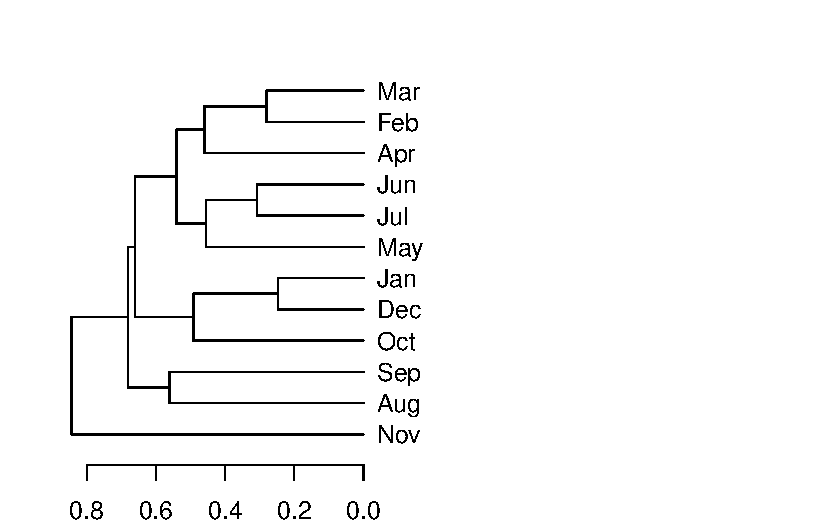
\includegraphics{report_nmds_files/figure-pdf/unnamed-chunk-23-1.pdf}

}

\end{figure}

\hypertarget{nmds-por-muxeas}{%
\subsection{NMDS POR MÊS}\label{nmds-por-muxeas}}

\begin{Shaded}
\begin{Highlighting}[]
\NormalTok{data\_nmds }\OtherTok{\textless{}{-}}
\NormalTok{  df }\SpecialCharTok{\%\textgreater{}\%}
  \FunctionTok{group\_by}\NormalTok{(Espécie, Localidade, Mês) }\SpecialCharTok{\%\textgreater{}\%}
  \FunctionTok{summarise}\NormalTok{(}\AttributeTok{abund =} \FunctionTok{n}\NormalTok{()) }\SpecialCharTok{\%\textgreater{}\%}
  \FunctionTok{pivot\_wider}\NormalTok{(}\AttributeTok{names\_from =}\NormalTok{ Espécie, }\AttributeTok{values\_from =}\NormalTok{ abund) }\SpecialCharTok{\%\textgreater{}\%}\FunctionTok{replace}\NormalTok{(}\FunctionTok{is.na}\NormalTok{(.), }\DecValTok{0}\NormalTok{)}
\end{Highlighting}
\end{Shaded}

\begin{verbatim}
`summarise()` has grouped output by 'Espécie', 'Localidade'. You can override
using the `.groups` argument.
\end{verbatim}

\begin{Shaded}
\begin{Highlighting}[]
\NormalTok{run\_nmds }\OtherTok{\textless{}{-}} 
\NormalTok{  data\_nmds}

\NormalTok{run\_nmds}\SpecialCharTok{$}\NormalTok{Localidade }\OtherTok{\textless{}{-}} \ConstantTok{NULL}
\NormalTok{run\_nmds}\SpecialCharTok{$}\NormalTok{Mês }\OtherTok{\textless{}{-}} \ConstantTok{NULL}

\NormalTok{dist\_bray }\OtherTok{\textless{}{-}} 
  \FunctionTok{vegdist}\NormalTok{(run\_nmds, }\AttributeTok{method =} \StringTok{"bray"}\NormalTok{, }\AttributeTok{binary =} \ConstantTok{TRUE}\NormalTok{)}

\NormalTok{nmds }\OtherTok{\textless{}{-}} 
  \FunctionTok{metaMDS}\NormalTok{(dist\_bray)}
\end{Highlighting}
\end{Shaded}

\begin{verbatim}
Run 0 stress 0.1861927 
Run 1 stress 0.1855069 
... New best solution
... Procrustes: rmse 0.03151088  max resid 0.1500422 
Run 2 stress 0.197264 
Run 3 stress 0.1953318 
Run 4 stress 0.1957449 
Run 5 stress 0.2192477 
Run 6 stress 0.212594 
Run 7 stress 0.1929643 
Run 8 stress 0.2141381 
Run 9 stress 0.1862234 
Run 10 stress 0.2024845 
Run 11 stress 0.1863356 
Run 12 stress 0.2032869 
Run 13 stress 0.1913283 
Run 14 stress 0.189773 
Run 15 stress 0.2000325 
Run 16 stress 0.1903028 
Run 17 stress 0.1891826 
Run 18 stress 0.1862229 
Run 19 stress 0.1885152 
Run 20 stress 0.1856259 
... Procrustes: rmse 0.03657719  max resid 0.226048 
*** Best solution was not repeated -- monoMDS stopping criteria:
     3: no. of iterations >= maxit
    17: stress ratio > sratmax
\end{verbatim}

\begin{Shaded}
\begin{Highlighting}[]
\FunctionTok{scores}\NormalTok{(nmds)  }\SpecialCharTok{\%\textgreater{}\%}
  \FunctionTok{as\_tibble}\NormalTok{() }\SpecialCharTok{\%\textgreater{}\%}
  \FunctionTok{cbind}\NormalTok{(data\_nmds) }\SpecialCharTok{\%\textgreater{}\%}
  \FunctionTok{as\_tibble}\NormalTok{()}\SpecialCharTok{\%\textgreater{}\%}
  \FunctionTok{ggplot}\NormalTok{(}\FunctionTok{aes}\NormalTok{(}\AttributeTok{x =}\NormalTok{ NMDS1, }\AttributeTok{y =}\NormalTok{ NMDS2)) }\SpecialCharTok{+}
  \FunctionTok{geom\_point}\NormalTok{(}\FunctionTok{aes}\NormalTok{(}\AttributeTok{color =}\NormalTok{ Mês)) }\SpecialCharTok{+}
  \FunctionTok{stat\_ellipse}\NormalTok{(}\AttributeTok{geom =} \StringTok{"polygon"}\NormalTok{, }
               \FunctionTok{aes}\NormalTok{(}\AttributeTok{group =}\NormalTok{ Mês, }\AttributeTok{color =}\NormalTok{ Mês, }\AttributeTok{fill =}\NormalTok{ Mês), }\AttributeTok{alpha =} \FloatTok{0.3}\NormalTok{) }\SpecialCharTok{+}
  \FunctionTok{annotate}\NormalTok{(}\StringTok{"text"}\NormalTok{, }\AttributeTok{x =} \SpecialCharTok{{-}}\DecValTok{3}\NormalTok{, }\AttributeTok{y =} \FloatTok{2.5}\NormalTok{, }
           \AttributeTok{label =} \FunctionTok{paste0}\NormalTok{(}\StringTok{"stress: "}\NormalTok{, }\FunctionTok{format}\NormalTok{(nmds}\SpecialCharTok{$}\NormalTok{stress, }\AttributeTok{digits =} \DecValTok{3}\NormalTok{)), }\AttributeTok{hjust =} \DecValTok{0}\NormalTok{) }\SpecialCharTok{+}
  \FunctionTok{theme\_bw}\NormalTok{()}
\end{Highlighting}
\end{Shaded}

\begin{figure}[H]

{\centering 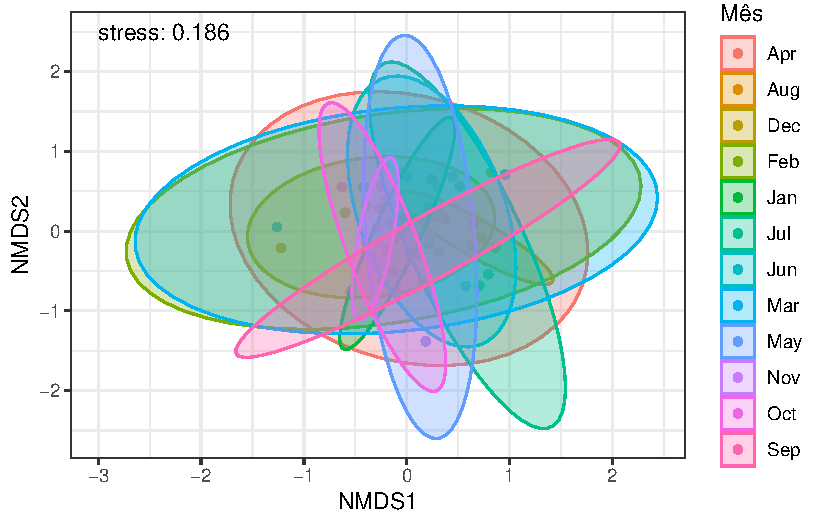
\includegraphics{report_nmds_files/figure-pdf/unnamed-chunk-24-1.pdf}

}

\end{figure}

\begin{Shaded}
\begin{Highlighting}[]
\CommentTok{\# Permanova}

\NormalTok{perm }\OtherTok{\textless{}{-}} \FunctionTok{adonis}\NormalTok{(dist\_bray}\SpecialCharTok{\textasciitilde{}}\NormalTok{data\_nmds}\SpecialCharTok{$}\NormalTok{Mês, }\AttributeTok{permutations =} \DecValTok{1000}\NormalTok{)}
\end{Highlighting}
\end{Shaded}

\begin{verbatim}
'adonis' will be deprecated: use 'adonis2' instead
\end{verbatim}

\begin{Shaded}
\begin{Highlighting}[]
\NormalTok{perm}\SpecialCharTok{$}\NormalTok{aov.tab}
\end{Highlighting}
\end{Shaded}

\begin{verbatim}
Permutation: free
Number of permutations: 1000

Terms added sequentially (first to last)

              Df SumsOfSqs MeanSqs F.Model      R2   Pr(>F)    
data_nmds$Mês 11    4.7305 0.43005   1.709 0.29466 0.000999 ***
Residuals     45   11.3234 0.25163         0.70534             
Total         56   16.0540                 1.00000             
---
Signif. codes:  0 '***' 0.001 '**' 0.01 '*' 0.05 '.' 0.1 ' ' 1
\end{verbatim}

\hypertarget{nmds-por-localidade}{%
\subsection{NMDS POR LOCALIDADE}\label{nmds-por-localidade}}

\begin{Shaded}
\begin{Highlighting}[]
\CommentTok{\# NMDS {-} 2 }

\NormalTok{data\_nmds }\OtherTok{\textless{}{-}} 
\NormalTok{  df }\SpecialCharTok{\%\textgreater{}\%}
  \FunctionTok{group\_by}\NormalTok{(Espécie, Localidade, Mês) }\SpecialCharTok{\%\textgreater{}\%}
  \FunctionTok{summarise}\NormalTok{(}\AttributeTok{abund =} \FunctionTok{n}\NormalTok{()) }\SpecialCharTok{\%\textgreater{}\%}
  \FunctionTok{pivot\_wider}\NormalTok{(}\AttributeTok{names\_from =}\NormalTok{ Espécie, }\AttributeTok{values\_from =}\NormalTok{ abund) }\SpecialCharTok{\%\textgreater{}\%}
  \FunctionTok{replace}\NormalTok{(}\FunctionTok{is.na}\NormalTok{(.), }\DecValTok{0}\NormalTok{)}
\end{Highlighting}
\end{Shaded}

\begin{verbatim}
`summarise()` has grouped output by 'Espécie', 'Localidade'. You can override
using the `.groups` argument.
\end{verbatim}

\begin{Shaded}
\begin{Highlighting}[]
\NormalTok{run\_nmds }\OtherTok{\textless{}{-}} 
\NormalTok{  data\_nmds}

\NormalTok{run\_nmds}\SpecialCharTok{$}\NormalTok{Localidade }\OtherTok{\textless{}{-}} \ConstantTok{NULL}
\NormalTok{run\_nmds}\SpecialCharTok{$}\NormalTok{Mês }\OtherTok{\textless{}{-}} \ConstantTok{NULL}

\NormalTok{dist\_bray }\OtherTok{\textless{}{-}} 
  \FunctionTok{vegdist}\NormalTok{(run\_nmds, }\AttributeTok{method =} \StringTok{"bray"}\NormalTok{, }\AttributeTok{binary =} \ConstantTok{TRUE}\NormalTok{)}

\NormalTok{nmds }\OtherTok{\textless{}{-}} 
  \FunctionTok{metaMDS}\NormalTok{(dist\_bray)}
\end{Highlighting}
\end{Shaded}

\begin{verbatim}
Run 0 stress 0.1861927 
Run 1 stress 0.1986203 
Run 2 stress 0.1896482 
Run 3 stress 0.1854072 
... New best solution
... Procrustes: rmse 0.05447529  max resid 0.2877863 
Run 4 stress 0.1862212 
Run 5 stress 0.19202 
Run 6 stress 0.1952903 
Run 7 stress 0.1896745 
Run 8 stress 0.1905095 
Run 9 stress 0.185625 
... Procrustes: rmse 0.008589263  max resid 0.03916664 
Run 10 stress 0.1891818 
Run 11 stress 0.1899779 
Run 12 stress 0.1853475 
... New best solution
... Procrustes: rmse 0.006399591  max resid 0.03728583 
Run 13 stress 0.1857359 
... Procrustes: rmse 0.06523239  max resid 0.4523092 
Run 14 stress 0.1885935 
Run 15 stress 0.1926246 
Run 16 stress 0.2172686 
Run 17 stress 0.1986962 
Run 18 stress 0.1899169 
Run 19 stress 0.2009015 
Run 20 stress 0.1903717 
*** Best solution was not repeated -- monoMDS stopping criteria:
     2: no. of iterations >= maxit
    18: stress ratio > sratmax
\end{verbatim}

\begin{Shaded}
\begin{Highlighting}[]
\FunctionTok{scores}\NormalTok{(nmds)  }\SpecialCharTok{\%\textgreater{}\%}
  \FunctionTok{as\_tibble}\NormalTok{() }\SpecialCharTok{\%\textgreater{}\%}
  \FunctionTok{cbind}\NormalTok{(data\_nmds) }\SpecialCharTok{\%\textgreater{}\%}
  \FunctionTok{as\_tibble}\NormalTok{()}\SpecialCharTok{\%\textgreater{}\%}
  \FunctionTok{ggplot}\NormalTok{(}\FunctionTok{aes}\NormalTok{(}\AttributeTok{x =}\NormalTok{ NMDS1, }\AttributeTok{y =}\NormalTok{ NMDS2)) }\SpecialCharTok{+}
  \FunctionTok{geom\_point}\NormalTok{(}\FunctionTok{aes}\NormalTok{(}\AttributeTok{color =}\NormalTok{ Localidade)) }\SpecialCharTok{+}
  \FunctionTok{stat\_ellipse}\NormalTok{(}\AttributeTok{geom =} \StringTok{"polygon"}\NormalTok{, }
               \FunctionTok{aes}\NormalTok{(}\AttributeTok{group =}\NormalTok{ Localidade, }\AttributeTok{color =}\NormalTok{ Localidade, }\AttributeTok{fill =}\NormalTok{ Localidade), }
               \AttributeTok{alpha =} \FloatTok{0.3}\NormalTok{) }\SpecialCharTok{+}
  \FunctionTok{annotate}\NormalTok{(}\StringTok{"text"}\NormalTok{, }\AttributeTok{x =} \SpecialCharTok{{-}}\DecValTok{5}\NormalTok{, }\AttributeTok{y =} \DecValTok{1}\NormalTok{, }
           \AttributeTok{label =} \FunctionTok{paste0}\NormalTok{(}\StringTok{"stress: "}\NormalTok{, }\FunctionTok{format}\NormalTok{(nmds}\SpecialCharTok{$}\NormalTok{stress, }\AttributeTok{digits =} \DecValTok{3}\NormalTok{)), }\AttributeTok{hjust =} \DecValTok{0}\NormalTok{) }\SpecialCharTok{+}
  \FunctionTok{theme\_bw}\NormalTok{()}
\end{Highlighting}
\end{Shaded}

\begin{figure}[H]

{\centering 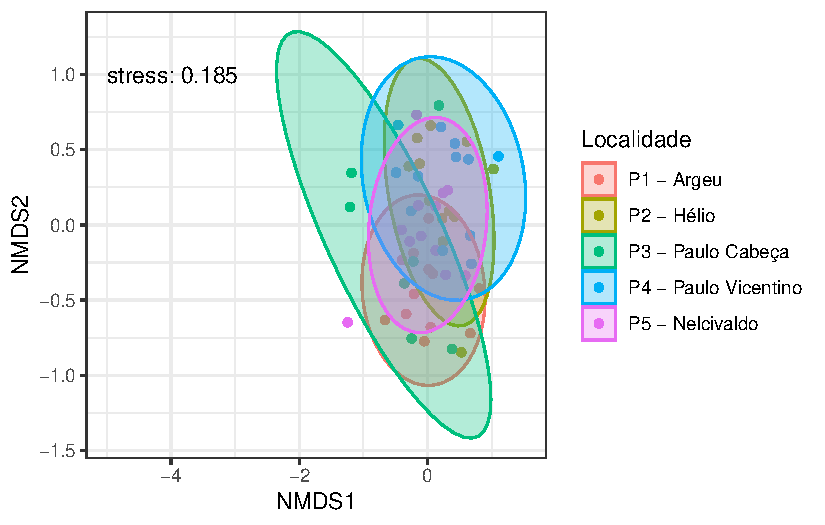
\includegraphics{report_nmds_files/figure-pdf/unnamed-chunk-26-1.pdf}

}

\end{figure}

\begin{Shaded}
\begin{Highlighting}[]
\CommentTok{\# Permanova}

\NormalTok{perm }\OtherTok{\textless{}{-}} \FunctionTok{adonis}\NormalTok{(dist\_bray}\SpecialCharTok{\textasciitilde{}}\NormalTok{data\_nmds}\SpecialCharTok{$}\NormalTok{Localidade, }\AttributeTok{permutations =} \DecValTok{1000}\NormalTok{)}
\end{Highlighting}
\end{Shaded}

\begin{verbatim}
'adonis' will be deprecated: use 'adonis2' instead
\end{verbatim}

\begin{Shaded}
\begin{Highlighting}[]
\NormalTok{perm}\SpecialCharTok{$}\NormalTok{aov.tab}
\end{Highlighting}
\end{Shaded}

\begin{verbatim}
Permutation: free
Number of permutations: 1000

Terms added sequentially (first to last)

                     Df SumsOfSqs MeanSqs F.Model      R2   Pr(>F)    
data_nmds$Localidade  4    3.3708 0.84271   3.455 0.20997 0.000999 ***
Residuals            52   12.6832 0.24391         0.79003             
Total                56   16.0540                 1.00000             
---
Signif. codes:  0 '***' 0.001 '**' 0.01 '*' 0.05 '.' 0.1 ' ' 1
\end{verbatim}

\hypertarget{nmds-por-armadilha}{%
\subsection{NMDS POR ARMADILHA}\label{nmds-por-armadilha}}

\begin{Shaded}
\begin{Highlighting}[]
\CommentTok{\# NMDS {-} 3 }

\NormalTok{data\_nmds }\OtherTok{\textless{}{-}} 
\NormalTok{  df }\SpecialCharTok{\%\textgreater{}\%}
  \FunctionTok{group\_by}\NormalTok{(Espécie, Armadilha, Localidade) }\SpecialCharTok{\%\textgreater{}\%}
  \FunctionTok{summarise}\NormalTok{(}\AttributeTok{abund =} \FunctionTok{n}\NormalTok{()) }\SpecialCharTok{\%\textgreater{}\%}
  \FunctionTok{pivot\_wider}\NormalTok{(}\AttributeTok{names\_from =}\NormalTok{ Espécie, }\AttributeTok{values\_from =}\NormalTok{ abund) }\SpecialCharTok{\%\textgreater{}\%}
  \FunctionTok{replace}\NormalTok{(}\FunctionTok{is.na}\NormalTok{(.), }\DecValTok{0}\NormalTok{)}
\end{Highlighting}
\end{Shaded}

\begin{verbatim}
`summarise()` has grouped output by 'Espécie', 'Armadilha'. You can override
using the `.groups` argument.
\end{verbatim}

\begin{Shaded}
\begin{Highlighting}[]
\NormalTok{run\_nmds }\OtherTok{\textless{}{-}} 
\NormalTok{  data\_nmds}

\NormalTok{run\_nmds}\SpecialCharTok{$}\NormalTok{Armadilha }\OtherTok{\textless{}{-}} \ConstantTok{NULL}
\NormalTok{run\_nmds}\SpecialCharTok{$}\NormalTok{Localidade }\OtherTok{\textless{}{-}} \ConstantTok{NULL}
\NormalTok{run\_nmds}\SpecialCharTok{$}\NormalTok{Mês }\OtherTok{\textless{}{-}} \ConstantTok{NULL}

\NormalTok{dist\_bray }\OtherTok{\textless{}{-}} 
  \FunctionTok{vegdist}\NormalTok{(run\_nmds, }\AttributeTok{method =} \StringTok{"bray"}\NormalTok{, }\AttributeTok{binary =} \ConstantTok{TRUE}\NormalTok{)}

\NormalTok{nmds }\OtherTok{\textless{}{-}} 
  \FunctionTok{metaMDS}\NormalTok{(dist\_bray)}
\end{Highlighting}
\end{Shaded}

\begin{verbatim}
Run 0 stress 0.155153 
Run 1 stress 0.1419521 
... New best solution
... Procrustes: rmse 0.2192153  max resid 0.5369558 
Run 2 stress 0.1730855 
Run 3 stress 0.1795324 
Run 4 stress 0.1550805 
Run 5 stress 0.1542007 
Run 6 stress 0.189781 
Run 7 stress 0.1550807 
Run 8 stress 0.1551526 
Run 9 stress 0.2465421 
Run 10 stress 0.1551528 
Run 11 stress 0.1542006 
Run 12 stress 0.1551527 
Run 13 stress 0.1419517 
... New best solution
... Procrustes: rmse 0.001353331  max resid 0.002532189 
... Similar to previous best
Run 14 stress 0.1419518 
... Procrustes: rmse 8.1971e-05  max resid 0.0001550068 
... Similar to previous best
Run 15 stress 0.1551527 
Run 16 stress 0.1419521 
... Procrustes: rmse 0.001367355  max resid 0.002559475 
... Similar to previous best
Run 17 stress 0.1795322 
Run 18 stress 0.1419519 
... Procrustes: rmse 0.001261296  max resid 0.002370973 
... Similar to previous best
Run 19 stress 0.1730855 
Run 20 stress 0.1551526 
*** Best solution repeated 4 times
\end{verbatim}

\begin{Shaded}
\begin{Highlighting}[]
\FunctionTok{scores}\NormalTok{(nmds)  }\SpecialCharTok{\%\textgreater{}\%}
  \FunctionTok{as\_tibble}\NormalTok{() }\SpecialCharTok{\%\textgreater{}\%}
  \FunctionTok{cbind}\NormalTok{(data\_nmds) }\SpecialCharTok{\%\textgreater{}\%}
  \FunctionTok{as\_tibble}\NormalTok{()}\SpecialCharTok{\%\textgreater{}\%}
  \FunctionTok{ggplot}\NormalTok{(}\FunctionTok{aes}\NormalTok{(}\AttributeTok{x =}\NormalTok{ NMDS1, }\AttributeTok{y =}\NormalTok{ NMDS2)) }\SpecialCharTok{+}
  \FunctionTok{geom\_point}\NormalTok{(}\FunctionTok{aes}\NormalTok{(}\AttributeTok{color =}\NormalTok{ Armadilha)) }\SpecialCharTok{+}
  \FunctionTok{stat\_ellipse}\NormalTok{(}\AttributeTok{geom =} \StringTok{"polygon"}\NormalTok{, }
               \FunctionTok{aes}\NormalTok{(}\AttributeTok{group =}\NormalTok{ Armadilha, }\AttributeTok{color =}\NormalTok{ Armadilha, }\AttributeTok{fill =}\NormalTok{ Armadilha), }
               \AttributeTok{alpha =} \FloatTok{0.3}\NormalTok{) }\SpecialCharTok{+}
  \FunctionTok{annotate}\NormalTok{(}\StringTok{"text"}\NormalTok{, }\AttributeTok{x =} \SpecialCharTok{{-}}\FloatTok{1.5}\NormalTok{, }\AttributeTok{y =} \FloatTok{2.5}\NormalTok{, }
           \AttributeTok{label =} \FunctionTok{paste0}\NormalTok{(}\StringTok{"stress: "}\NormalTok{, }\FunctionTok{format}\NormalTok{(nmds}\SpecialCharTok{$}\NormalTok{stress, }\AttributeTok{digits =} \DecValTok{3}\NormalTok{)), }\AttributeTok{hjust =} \DecValTok{0}\NormalTok{) }\SpecialCharTok{+}
  \FunctionTok{theme\_bw}\NormalTok{()}
\end{Highlighting}
\end{Shaded}

\begin{figure}[H]

{\centering 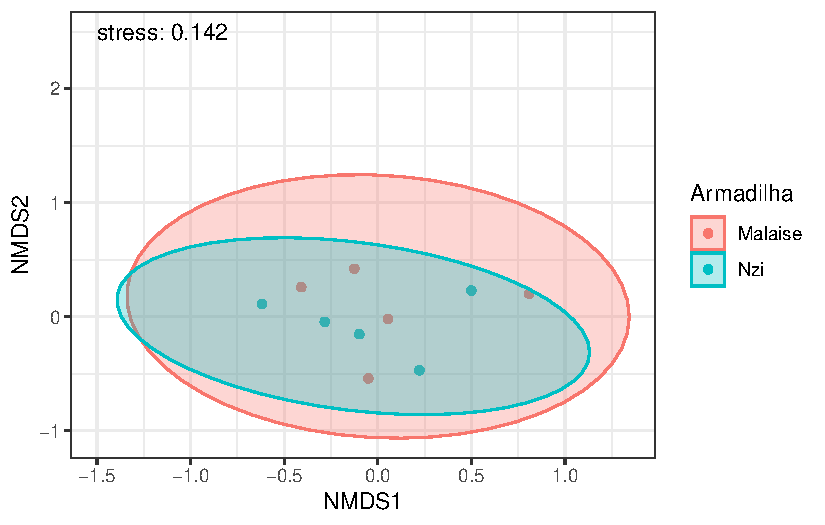
\includegraphics{report_nmds_files/figure-pdf/unnamed-chunk-28-1.pdf}

}

\end{figure}

\begin{Shaded}
\begin{Highlighting}[]
\NormalTok{perm }\OtherTok{\textless{}{-}} \FunctionTok{adonis}\NormalTok{(dist\_bray}\SpecialCharTok{\textasciitilde{}}\NormalTok{data\_nmds}\SpecialCharTok{$}\NormalTok{Armadilha, }\AttributeTok{permutations =} \DecValTok{1000}\NormalTok{)}
\end{Highlighting}
\end{Shaded}

\begin{verbatim}
'adonis' will be deprecated: use 'adonis2' instead
\end{verbatim}

\begin{Shaded}
\begin{Highlighting}[]
\NormalTok{perm}\SpecialCharTok{$}\NormalTok{aov.tab}
\end{Highlighting}
\end{Shaded}

\begin{verbatim}
Permutation: free
Number of permutations: 1000

Terms added sequentially (first to last)

                    Df SumsOfSqs MeanSqs F.Model      R2 Pr(>F)
data_nmds$Armadilha  1   0.24668 0.24668  1.5132 0.15906 0.1958
Residuals            8   1.30417 0.16302         0.84094       
Total                9   1.55085                 1.00000       
\end{verbatim}

\hypertarget{nmds-por-ambiente}{%
\subsection{NMDS POR AMBIENTE}\label{nmds-por-ambiente}}

\begin{Shaded}
\begin{Highlighting}[]
\CommentTok{\# NMDS {-} 3 }

\NormalTok{data\_nmds }\OtherTok{\textless{}{-}} 
\NormalTok{  df }\SpecialCharTok{\%\textgreater{}\%}
  \FunctionTok{group\_by}\NormalTok{(Espécie, Ambiente, Localidade) }\SpecialCharTok{\%\textgreater{}\%}
  \FunctionTok{summarise}\NormalTok{(}\AttributeTok{abund =} \FunctionTok{n}\NormalTok{()) }\SpecialCharTok{\%\textgreater{}\%}
  \FunctionTok{pivot\_wider}\NormalTok{(}\AttributeTok{names\_from =}\NormalTok{ Espécie, }\AttributeTok{values\_from =}\NormalTok{ abund) }\SpecialCharTok{\%\textgreater{}\%}
  \FunctionTok{replace}\NormalTok{(}\FunctionTok{is.na}\NormalTok{(.), }\DecValTok{0}\NormalTok{)}
\end{Highlighting}
\end{Shaded}

\begin{verbatim}
`summarise()` has grouped output by 'Espécie', 'Ambiente'. You can override
using the `.groups` argument.
\end{verbatim}

\begin{Shaded}
\begin{Highlighting}[]
\NormalTok{run\_nmds }\OtherTok{\textless{}{-}} 
\NormalTok{  data\_nmds}

\NormalTok{run\_nmds}\SpecialCharTok{$}\NormalTok{Ambiente }\OtherTok{\textless{}{-}} \ConstantTok{NULL}
\NormalTok{run\_nmds}\SpecialCharTok{$}\NormalTok{Localidade }\OtherTok{\textless{}{-}} \ConstantTok{NULL}
\NormalTok{run\_nmds}\SpecialCharTok{$}\NormalTok{Mês }\OtherTok{\textless{}{-}} \ConstantTok{NULL}

\NormalTok{dist\_bray }\OtherTok{\textless{}{-}} 
  \FunctionTok{vegdist}\NormalTok{(run\_nmds, }\AttributeTok{method =} \StringTok{"bray"}\NormalTok{, }\AttributeTok{binary =} \ConstantTok{TRUE}\NormalTok{)}

\NormalTok{nmds }\OtherTok{\textless{}{-}} 
  \FunctionTok{metaMDS}\NormalTok{(dist\_bray)}
\end{Highlighting}
\end{Shaded}

\begin{verbatim}
Run 0 stress 0.04954689 
Run 1 stress 0.04954682 
... New best solution
... Procrustes: rmse 5.342142e-05  max resid 0.000124007 
... Similar to previous best
Run 2 stress 0.06035446 
Run 3 stress 0.04954681 
... New best solution
... Procrustes: rmse 0.0003624999  max resid 0.00087586 
... Similar to previous best
Run 4 stress 0.04954679 
... New best solution
... Procrustes: rmse 0.0003105556  max resid 0.0007514486 
... Similar to previous best
Run 5 stress 0.0495468 
... Procrustes: rmse 2.75829e-05  max resid 5.528266e-05 
... Similar to previous best
Run 6 stress 0.1465096 
Run 7 stress 0.0495468 
... Procrustes: rmse 3.231599e-05  max resid 7.354997e-05 
... Similar to previous best
Run 8 stress 0.0495468 
... Procrustes: rmse 0.0002895633  max resid 0.0006979861 
... Similar to previous best
Run 9 stress 0.04954675 
... New best solution
... Procrustes: rmse 0.0001049378  max resid 0.0002476308 
... Similar to previous best
Run 10 stress 0.04954678 
... Procrustes: rmse 9.529043e-05  max resid 0.0002245183 
... Similar to previous best
Run 11 stress 0.04954684 
... Procrustes: rmse 0.0002425671  max resid 0.0005902716 
... Similar to previous best
Run 12 stress 0.1465098 
Run 13 stress 0.04954679 
... Procrustes: rmse 0.0001134803  max resid 0.0002692882 
... Similar to previous best
Run 14 stress 0.04954677 
... Procrustes: rmse 0.0001500963  max resid 0.0003653968 
... Similar to previous best
Run 15 stress 0.04954681 
... Procrustes: rmse 0.0002056867  max resid 0.0004984323 
... Similar to previous best
Run 16 stress 0.06035461 
Run 17 stress 0.0495468 
... Procrustes: rmse 0.0001856151  max resid 0.000451163 
... Similar to previous best
Run 18 stress 0.04954679 
... Procrustes: rmse 0.0001015826  max resid 0.0002392312 
... Similar to previous best
Run 19 stress 0.04954689 
... Procrustes: rmse 0.0002932971  max resid 0.0007117018 
... Similar to previous best
Run 20 stress 0.04954682 
... Procrustes: rmse 0.0002211859  max resid 0.0005373356 
... Similar to previous best
*** Best solution repeated 10 times
\end{verbatim}

\begin{Shaded}
\begin{Highlighting}[]
\FunctionTok{scores}\NormalTok{(nmds)  }\SpecialCharTok{\%\textgreater{}\%}
  \FunctionTok{as\_tibble}\NormalTok{() }\SpecialCharTok{\%\textgreater{}\%}
  \FunctionTok{cbind}\NormalTok{(data\_nmds) }\SpecialCharTok{\%\textgreater{}\%}
  \FunctionTok{as\_tibble}\NormalTok{()}\SpecialCharTok{\%\textgreater{}\%}
  \FunctionTok{ggplot}\NormalTok{(}\FunctionTok{aes}\NormalTok{(}\AttributeTok{x =}\NormalTok{ NMDS1, }\AttributeTok{y =}\NormalTok{ NMDS2)) }\SpecialCharTok{+}
  \FunctionTok{geom\_point}\NormalTok{(}\FunctionTok{aes}\NormalTok{(}\AttributeTok{color =}\NormalTok{ Ambiente)) }\SpecialCharTok{+}
  \FunctionTok{stat\_ellipse}\NormalTok{(}\AttributeTok{geom =} \StringTok{"polygon"}\NormalTok{, }
               \FunctionTok{aes}\NormalTok{(}\AttributeTok{group =}\NormalTok{ Ambiente, }\AttributeTok{color =}\NormalTok{ Ambiente, }\AttributeTok{fill =}\NormalTok{ Ambiente), }
               \AttributeTok{alpha =} \FloatTok{0.3}\NormalTok{) }\SpecialCharTok{+}
  \FunctionTok{annotate}\NormalTok{(}\StringTok{"text"}\NormalTok{, }\AttributeTok{x =} \SpecialCharTok{{-}}\FloatTok{2.5}\NormalTok{, }\AttributeTok{y =} \FloatTok{1.5}\NormalTok{, }
           \AttributeTok{label =} \FunctionTok{paste0}\NormalTok{(}\StringTok{"stress: "}\NormalTok{, }\FunctionTok{format}\NormalTok{(nmds}\SpecialCharTok{$}\NormalTok{stress, }\AttributeTok{digits =} \DecValTok{3}\NormalTok{)), }\AttributeTok{hjust =} \DecValTok{0}\NormalTok{) }\SpecialCharTok{+}
  \FunctionTok{theme\_bw}\NormalTok{()}
\end{Highlighting}
\end{Shaded}

\begin{figure}[H]

{\centering 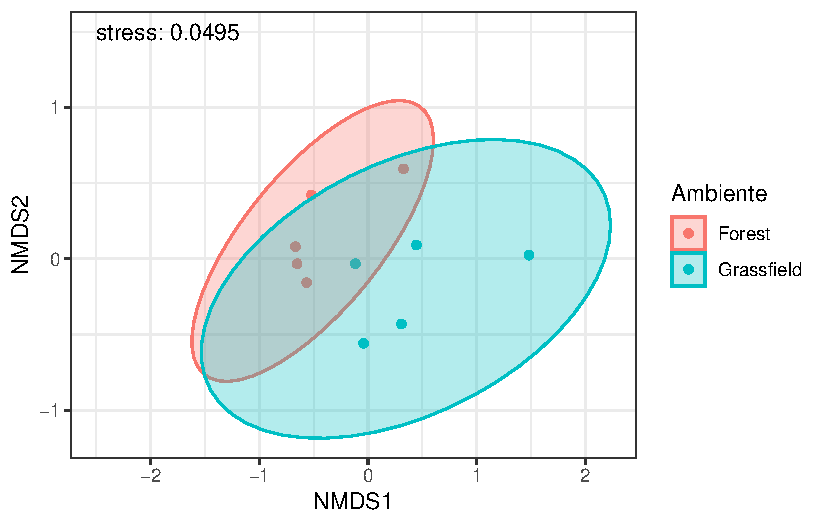
\includegraphics{report_nmds_files/figure-pdf/unnamed-chunk-30-1.pdf}

}

\end{figure}

\begin{Shaded}
\begin{Highlighting}[]
\NormalTok{perm }\OtherTok{\textless{}{-}} \FunctionTok{adonis}\NormalTok{(dist\_bray}\SpecialCharTok{\textasciitilde{}}\NormalTok{data\_nmds}\SpecialCharTok{$}\NormalTok{Ambiente, }\AttributeTok{permutations =} \DecValTok{1000}\NormalTok{)}
\end{Highlighting}
\end{Shaded}

\begin{verbatim}
'adonis' will be deprecated: use 'adonis2' instead
\end{verbatim}

\begin{Shaded}
\begin{Highlighting}[]
\NormalTok{perm}\SpecialCharTok{$}\NormalTok{aov.tab}
\end{Highlighting}
\end{Shaded}

\begin{verbatim}
Permutation: free
Number of permutations: 1000

Terms added sequentially (first to last)

                   Df SumsOfSqs MeanSqs F.Model      R2   Pr(>F)   
data_nmds$Ambiente  1   0.49038 0.49038  2.8469 0.26246 0.006993 **
Residuals           8   1.37802 0.17225         0.73754            
Total               9   1.86840                 1.00000            
---
Signif. codes:  0 '***' 0.001 '**' 0.01 '*' 0.05 '.' 0.1 ' ' 1
\end{verbatim}



\end{document}
